\chapter{光滑优化}
\label{chap:opt-smooth}

设想要最小化$f(\bm x)=\tfrac12(x_1^2+16x_2^2)$，从$\bm x^{(0)}=(2,2)^\top$出发。最小点显然在原点，但算法看不到整张等高线图，它在当前点只能读到目标值$34$和梯度$(2,32)^\top$。负梯度几乎竖直地指向$x_2$方向，而从$(2,2)^\top$通往原点的直线却沿对角线；沿负梯度走多远也没有现成答案：走$1/16$个单位梯度长度时目标降到约$1.76$，走$1/8$时第二个坐标只是换了符号，再长一点就会越过谷底、越走越高。仅凭一个点上的局部信息，怎样决定方向和步长？怎样保证每一步确实让目标下降？什么时候值得付出更多计算去读取曲率？最后返回的点又有多准确、花了多少代价？

本章研究有限维、无约束、目标可微的问题$\min_{\bm x\in\mathbb R^d}f(\bm x)$。学习目标有三层。第一，说清局部信息在什么条件下能控制有限位移后的目标变化，并由此推导梯度下降、线搜索、预条件与动量等一阶方法，写出每种方法的输入、更新、接受与停止规则及其收敛保证。第二，理解曲率怎样构造更好的局部模型：牛顿法、修正牛顿法、信赖域、Newton--CG、拟牛顿与立方正则化各自解决局部模型的哪一个缺陷，又为此付出什么。第三，在非凸目标和有限精度计算下，区分驻点、鞍点与局部最小点，区分算法求解误差与问题自身对数据的敏感性，并在同一精度标准下比较方法的总计算成本。第~\ref{chap:optimization}章已经建立了凸性、强凸性和一阶、二阶最优条件，本章直接使用这些结论。

各节的先后由一个共同依据串起来：目标在一点附近能用怎样的局部模型代替，以及模型与真实目标差多少。第一节用梯度Lipschitz条件给出二次上界，它同时回答了“往哪走”和“走多远”；第二节只用梯度和有限历史，比较固定步长、线搜索、坐标变换与动量；第三节把曲率放进模型，处理模型不正定、不可信和太贵的问题；第四节转向非凸目标，研究下降方法可能停在哪里，以及怎样利用负曲率离开鞍点。前四节都在固定的问题上构造算法，第五节固定精度标准，比较速度、成本与计算误差；第六节改变问题本身的数据，研究即使精确求解，最优解又会移动多少。本章所用的梯度都是同一个确定目标的精确梯度，抽样梯度与随历史变化的自适应缩放留到第~\ref{chap:opt-stochastic-block}章，残差结构专用的Gauss--Newton与Levenberg--Marquardt方法留到第~\ref{chap:opt-function-fitting}章。

\section{光滑目标与局部上界}
\label{sec:opt-smooth-local-bounds}

梯度只描述目标在当前点的一阶变化率，而算法每一步都要走出有限长度。一阶Taylor展开$f(\bm x+\bm p)\approx f(\bm x)+\langle\nabla f(\bm x),\bm p\rangle$在$\bm p\to\bm0$时成立，却没有说$\bm p$多大时误差可以忽略。本节回答局部导数信息怎样控制有限位移后的目标变化：先给梯度的变化速度规定上限，得到一阶模型的二次误差界；再把候选位移代入这个界，看出方向与步长各自承担什么作用。后面各节的求步规则和接受规则，都以这里的上界为共同依据。

本章反复使用一个二维例子：
\begin{equation}
\label{eq:opt-smooth-common-quadratic}
  f(\bm x)=\frac12\bigl(x_1^2+16x_2^2\bigr)=\frac12\bm x^\top\bm H\bm x,\qquad
  \bm H=\operatorname{diag}(1,16),\qquad
  \bm x^{(0)}=(2,2)^\top.
\end{equation}
它的最小点是原点，$f^\star=0$，初始目标值$f(\bm x^{(0)})=34$，梯度$\nabla f(\bm x)=\bm H\bm x=(x_1,16x_2)^\top$。两个坐标方向的曲率相差$16$倍，这个差别足以暴露本章讨论的大部分现象，而每一步又都能手算。

\subsection{梯度光滑性}
\label{sec:opt-smooth-lipschitz-gradient}

在共同例中，从某点沿$x_1$方向移动单位长度，梯度改变$(1,0)^\top$；沿$x_2$方向移动单位长度，梯度改变$(0,16)^\top$。同样长的位移，在陡的方向上使梯度改变得多，梯度变得越快，一阶近似失效得也越快。一般地，$\nabla f(\bm u)-\nabla f(\bm v)=\bm H(\bm u-\bm v)$，所以
\[
  \lVert\nabla f(\bm u)-\nabla f(\bm v)\rVert_2\leq\lVert\bm H\rVert_2\lVert\bm u-\bm v\rVert_2=16\lVert\bm u-\bm v\rVert_2,
\]
等号在$\bm u-\bm v$平行于$x_2$轴时取得。数字$16$是“每移动单位距离，梯度最多改变多少”的上限。对一般目标，我们要求同样的上限在关心的区域内统一存在。

\begin{definition}[梯度Lipschitz条件与$L$光滑]
\label{def:opt-smooth-l-smooth}
设$U\subseteq\mathbb R^d$，$f$在包含$U$的开集上可微，$L\geq0$。若对所有$\bm u,\bm v\in U$都有
\[
  \lVert\nabla f(\bm u)-\nabla f(\bm v)\rVert_2\leq L\lVert\bm u-\bm v\rVert_2,
\]
就说$\nabla f$在$U$上是$L$-Lipschitz的，也称$f$在$U$上\term{$L$光滑}（$L$-smooth）。$U=\mathbb R^d$时简称$f$为$L$光滑。
\end{definition}

这个条件比“可微”和“梯度连续”都强，三者需要分开。$f(x)=\tfrac23|x|^{3/2}$在$\mathbb R$上可微，导数$f'(x)=\operatorname{sign}(x)|x|^{1/2}$也连续，但$|f'(x)-f'(0)|/|x|=|x|^{-1/2}$在$x\to0$时无界，所以在包含原点的任何区间上都不存在光滑常数。$f(x)=x^4$无穷次可微，却因$f''(x)=12x^2$无界而不是全局$L$光滑；限制在$[-R,R]$上，由中值定理$|f'(u)-f'(v)|\leq12R^2|u-v|$，常数$12R^2$随区域变大。所以说一个目标“光滑”时，必须同时说明常数$L$和它成立的区域。

对二阶连续可微的目标，常数可以从Hessian读出。若$U$是凸开集且$\lVert\nabla^2f(\bm z)\rVert_2\leq L$对所有$\bm z\in U$成立，则对$\bm u,\bm v\in U$，沿线段积分得
\[
  \nabla f(\bm u)-\nabla f(\bm v)=\int_0^1\nabla^2f\bigl(\bm v+s(\bm u-\bm v)\bigr)(\bm u-\bm v)\,\mathrm ds,
\]
取范数即得$\lVert\nabla f(\bm u)-\nabla f(\bm v)\rVert_2\leq L\lVert\bm u-\bm v\rVert_2$。这里用到线段留在$U$中，这正是要求$U$为凸集的原因。对实对称矩阵，$\lVert\nabla^2f(\bm z)\rVert_2$等于其特征值绝对值的最大者；二次目标$\tfrac12\bm x^\top\bm H\bm x$的最小光滑常数就是$\bm H$的谱半径$\max_i|\lambda_i(\bm H)|$。实对称矩阵的正交谱分解与谱范数可参考\BookChapterRef{chap:linear-analysis}{卷一“谱和奇异值”章}；本章只用“二次型$\bm v^\top\bm H\bm v$介于最小与最大特征值乘$\lVert\bm v\rVert_2^2$之间”这一结论。

\paragraph{一阶模型的余项界}
有了梯度变化的上限，就能控制一阶模型与真实目标之差。

\begin{lemma}[下降引理]
\label{lem:opt-smooth-descent-lemma}
设$f$在凸集$U$上$L$光滑，$\bm x,\bm x+\bm p\in U$。则
\begin{equation}
\label{eq:opt-smooth-descent-lemma}
  \bigl|f(\bm x+\bm p)-f(\bm x)-\langle\nabla f(\bm x),\bm p\rangle\bigr|\leq\frac L2\lVert\bm p\rVert_2^2 .
\end{equation}
特别地，$f(\bm x+\bm p)\leq f(\bm x)+\langle\nabla f(\bm x),\bm p\rangle+\tfrac L2\lVert\bm p\rVert_2^2$。
\end{lemma}

\begin{proof}
令$\phi(s)=f(\bm x+s\bm p)$，$s\in[0,1]$。由于线段在$U$中，$\phi$可微且$\phi'(s)=\langle\nabla f(\bm x+s\bm p),\bm p\rangle$连续，于是
\[
  f(\bm x+\bm p)-f(\bm x)-\langle\nabla f(\bm x),\bm p\rangle
  =\int_0^1\bigl\langle\nabla f(\bm x+s\bm p)-\nabla f(\bm x),\bm p\bigr\rangle\,\mathrm ds .
\]
由Cauchy--Schwarz不等式和梯度Lipschitz条件，被积函数的绝对值不超过$\lVert\nabla f(\bm x+s\bm p)-\nabla f(\bm x)\rVert_2\lVert\bm p\rVert_2\leq Ls\lVert\bm p\rVert_2^2$，对$s$积分得$\tfrac L2\lVert\bm p\rVert_2^2$。
\end{proof}

引理的上半部分称为\term{下降引理}（descent lemma），因为后面会用它证明目标下降。它说：在当前点放一个开口向上、曲率为$L$的抛物面，这个抛物面在$\bm x$处与$f$相切，并且在整个$U$上盖住$f$；另一个开口向下的抛物面从下方托住$f$。图~\ref{fig:opt-smooth-upper-bound}画出了一维情形。$f(x)=\log(1+x^2)$的二阶导数$f''(x)=2(1-x^2)/(1+x^2)^2$取值在$[-1/4,2]$中，故$L=2$；在$x^{(0)}=1.5$处，两条抛物线夹住整条曲线。式~\eqref{eq:opt-smooth-descent-lemma}的证明只用到线段上的梯度，所以当$L$只在某个区域内成立时，候选点和连接它的线段都必须留在该区域中。

\begin{figure}[htbp]
  \centering
  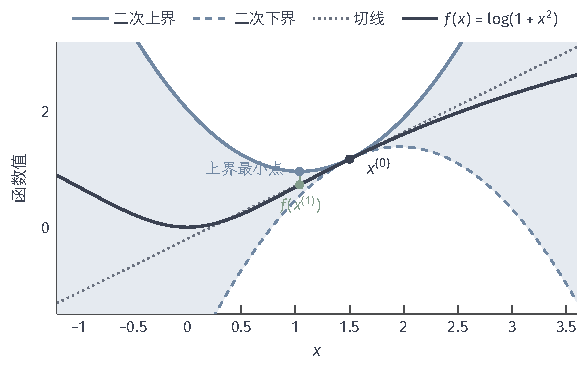
\includegraphics[width=99.5mm]{figures/03-optimization-evolution-and-signals/01-optimization/tikz/c3-quadratic-upper-bound/figure.pdf}
  \caption{一维目标$f(x)=\log(1+x^2)$在$x^{(0)}=1.5$处的二次上界与二次下界（$L=2$）。蓝色实线是$f(x^{(0)})+f'(x^{(0)})(x-x^{(0)})+(x-x^{(0)})^2$，虚线是把最后一项换成负号的下界，浅蓝区域夹住了黑色曲线。上界的最小点在$x^{(1)}=x^{(0)}-f'(x^{(0)})/L\approx1.038$，上界在该处的值约$0.966$；真实目标$f(x^{(1)})\approx0.732$（绿点）更低。}
  \label{fig:opt-smooth-upper-bound}
\end{figure}

\paragraph{共同例中的常数}
对式~\eqref{eq:opt-smooth-common-quadratic}，余项恰为$\tfrac12\bm p^\top\bm H\bm p=\tfrac12(p_1^2+16p_2^2)$，介于$\tfrac12\lVert\bm p\rVert_2^2$与$8\lVert\bm p\rVert_2^2$之间。$L=16$给出的上界只在$\bm p$平行于$x_2$轴时取等号；沿$x_1$方向，真实余项只有上界的$1/16$。这就是后面一切困难的来源：一个统一的常数必须照顾最陡的方向，因而对平坦方向过于保守。最小特征值$1$在这里对应第~\ref{chap:optimization}章的强凸常数$\mu$，它给出一阶模型误差的下界；本章记$\kappa=L/\mu$为条件数，共同例中$\kappa=16$。

\subsection{下降方向与模型上界}
\label{sec:opt-smooth-descent-direction}

有了上界，就可以把“选一个更新”拆成两个问题：沿哪个方向走，以及走多远。本小节先说明方向正确是什么意思，再说明为什么方向正确还不够。

\paragraph{下降方向}
在$\bm x$处沿方向$\bm d$的方向导数是$\langle\nabla f(\bm x),\bm d\rangle$。若它为负，就称$\bm d$为\term{下降方向}（descent direction）。由方向导数的定义，$f(\bm x+\eta\bm d)=f(\bm x)+\eta\langle\nabla f(\bm x),\bm d\rangle+o(\eta)$，所以存在$\bar\eta>0$，使$0<\eta<\bar\eta$时$f(\bm x+\eta\bm d)<f(\bm x)$。这个$\bar\eta$只是存在，定义没有告诉我们它有多大。负梯度$\bm d=-\nabla f(\bm x)$在非驻点处总是下降方向，因为$\langle\nabla f(\bm x),-\nabla f(\bm x)\rangle=-\lVert\nabla f(\bm x)\rVert_2^2<0$；任何与负梯度夹角小于直角的方向也是。

\paragraph{方向与步长的分工}
把位移$\eta\bm d$代入下降引理，记$\bm g=\nabla f(\bm x)$：
\begin{equation}
\label{eq:opt-smooth-direction-step}
  f(\bm x+\eta\bm d)\leq f(\bm x)+\eta\langle\bm g,\bm d\rangle+\frac{L\eta^2}{2}\lVert\bm d\rVert_2^2 .
\end{equation}
右边是$\eta$的二次函数。一次项由方向决定：只有$\langle\bm g,\bm d\rangle<0$时，小步长才能使右边低于$f(\bm x)$。二次项由步长决定：只有$0<\eta<2|\langle\bm g,\bm d\rangle|/(L\lVert\bm d\rVert_2^2)$时右边才严格低于$f(\bm x)$。在$\eta=|\langle\bm g,\bm d\rangle|/(L\lVert\bm d\rVert_2^2)$处右边最小，保证的下降量为
\[
  \frac{\langle\bm g,\bm d\rangle^2}{2L\lVert\bm d\rVert_2^2}=\frac{\lVert\bm g\rVert_2^2\cos^2\theta}{2L},
\]
其中$\theta$是$\bm d$与$-\bm g$的夹角。方向越偏离负梯度，能保证的下降越少；而方向再好，步长超出范围也可能上升。一维例子就能看到后者：$f(x)=8x^2$的$L=16$，在$x=1$处负梯度方向$d=-16$是下降方向，但取$\eta=0.2$得到$x=1-3.2=-2.2$，$f(-2.2)=38.72>8=f(1)$。方向没有错，错在步长越过了曲率允许的范围。

\paragraph{二次模型生成更新}
把方向和步长合在一起考虑，可以直接对整个位移$\bm p$最小化上界：
\[
  \min_{\bm p}\ f(\bm x)+\langle\bm g,\bm p\rangle+\frac L2\lVert\bm p\rVert_2^2 ,
\]
对$\bm p$求梯度并令其为零得$\bm p=-\bm g/L$，这正是步长$1/L$的梯度步，保证的下降量为$\lVert\bm g\rVert_2^2/(2L)$。图~\ref{fig:opt-smooth-upper-bound}中蓝点就是一维的这一步：在“碗盖”的最低处落脚，真实目标只会更低。

这个推理可以推广。对任意对称正定矩阵$\bm B$，考虑二次模型
\begin{equation}
\label{eq:opt-smooth-quadratic-model}
  m_{\bm B}(\bm p)=f(\bm x)+\langle\bm g,\bm p\rangle+\frac12\bm p^\top\bm B\bm p .
\end{equation}
它有唯一最小点$\bm p=-\bm B^{-1}\bm g$，且$\langle\bm g,\bm p\rangle=-\bm g^\top\bm B^{-1}\bm g<0$（$\bm g\neq\bm0$），所以无论$\bm B$怎样取，只要正定，模型步都是下降方向。取$\bm B=L\bm I$得到梯度下降；取固定的$\bm B=\bm P^{-1}$得到第~\ref{sec:opt-smooth-preconditioning}小节的预条件梯度法；取Hessian得到牛顿法；用观测到的梯度变化拼出$\bm B$得到拟牛顿法。只有当$\bm B$在相关区域内“盖得住”目标的曲率时，例如$\bm B=L\bm I$，模型最小点才自动保证原目标下降；其他选择下，模型只是近似，还需要线搜索、信赖域等接受规则用原目标核验。后续各方法的差别，就在于怎样构造$\bm B$、怎样求解模型，以及怎样决定接受与否。

\section{梯度方法}
\label{sec:opt-smooth-gradient-methods}

上一节说明，在$L$光滑的目标上，步长$1/L$的负梯度步一定下降。本节研究只用梯度和少量历史，能把这个保证推进到什么程度。四个小节固定同一个问题和同一类评价标准，依次改变一个要素：先只改变步长的选法（固定步长或线搜索），再改变度量位移的坐标（预条件），最后让更新带上前几步的记忆（重球法与Nesterov方法）。每一种改变都写清算法维护的状态、一轮更新、接受或停止规则、所需条件与每轮代价。

\subsection{梯度下降与线搜索}
\label{sec:opt-smooth-gd-linesearch}

\term{梯度下降}（gradient descent）从初值出发，反复沿负梯度走一步：
\begin{equation}
\label{eq:opt-smooth-gd}
  \bm x^{(t+1)}=\bm x^{(t)}-\eta^{(t)}\nabla f(\bm x^{(t)}),\qquad t=0,1,2,\dots
\end{equation}
算法的状态只有当前点；每轮计算一次梯度，若要监控目标或使用线搜索，再计算若干次函数值。下面先研究已知光滑常数时的固定步长，再研究常数未知时怎样让函数值本身决定步长。

\begin{algorithm}[固定步长梯度下降]
\label{alg:opt-smooth-gd}
\begin{algorithmic}[1]
\Require 可微目标$f$，初值$\bm x^{(0)}$，步长$\eta>0$，梯度容差$\varepsilon>0$，最大轮数$T$
\Ensure 返回点$\hat{\bm x}$
\State $\hat{\bm x}\gets\bm x^{(0)}$
\For{$t=0,1,\dots,T-1$}
  \State $\bm g^{(t)}\gets\nabla f(\bm x^{(t)})$
  \If{$\lVert\bm g^{(t)}\rVert_2<\lVert\nabla f(\hat{\bm x})\rVert_2$} \State $\hat{\bm x}\gets\bm x^{(t)}$ \Comment{记录梯度最小的已访问点}\EndIf
  \If{$\lVert\bm g^{(t)}\rVert_2\leq\varepsilon$} \State \Return $\bm x^{(t)}$ \EndIf
  \State $\bm x^{(t+1)}\gets\bm x^{(t)}-\eta\,\bm g^{(t)}$
\EndFor
\State \Return $\hat{\bm x}$（凸目标也可返回最后一点$\bm x^{(T)}$）
\end{algorithmic}
\end{algorithm}

返回哪一个点要和随后的保证对应：非凸目标的保证只针对梯度最小的已访问点，凸目标的目标差保证针对最后一点。记录最佳点不需要额外的梯度计算，因为每轮已经算出了$\bm g^{(t)}$。

\paragraph{单步下降与驻点残差}
把$\bm p=-\eta\nabla f(\bm x)$代入下降引理~\eqref{eq:opt-smooth-descent-lemma}，记$\bm x^+=\bm x-\eta\nabla f(\bm x)$，得到
\begin{equation}
\label{eq:opt-smooth-gd-one-step}
  f(\bm x^+)\leq f(\bm x)-\eta\Bigl(1-\frac{L\eta}{2}\Bigr)\lVert\nabla f(\bm x)\rVert_2^2 .
\end{equation}
所以$0<\eta<2/L$时，每个非驻点处目标严格下降；系数$\eta(1-L\eta/2)$在$\eta=1/L$时最大，等于$1/(2L)$。单步下降还不能告诉我们何时接近驻点。若目标下有界，把各步下降累加起来，下降的总量受初值与下界之差限制，于是梯度不可能一直很大。

\begin{theorem}[非凸光滑目标上的梯度下降]
\label{thm:opt-smooth-gd-nonconvex}
设$f:\mathbb R^d\to\mathbb R$为$L$光滑（$L>0$），$f_{\inf}=\inf f>-\infty$，取固定步长$0<\eta<2/L$。则对任意初值和$T\geq1$，
\begin{equation}
\label{eq:opt-smooth-gd-nonconvex-rate}
  \min_{0\leq t<T}\lVert\nabla f(\bm x^{(t)})\rVert_2^2\leq\frac{f(\bm x^{(0)})-f_{\inf}}{T\,\eta(1-L\eta/2)} .
\end{equation}
取$\eta=1/L$时右边为$2L\bigl(f(\bm x^{(0)})-f_{\inf}\bigr)/T$，且$\nabla f(\bm x^{(t)})\to\bm0$。
\end{theorem}

\begin{proof}
对$t=0,\dots,T-1$把式~\eqref{eq:opt-smooth-gd-one-step}相加，左右两边的目标值逐项相消：
\[
  \eta\Bigl(1-\frac{L\eta}2\Bigr)\sum_{t=0}^{T-1}\lVert\nabla f(\bm x^{(t)})\rVert_2^2\leq f(\bm x^{(0)})-f(\bm x^{(T)})\leq f(\bm x^{(0)})-f_{\inf}.
\]
左边的和不小于$T$乘以其中最小的一项，除以$T\eta(1-L\eta/2)$即得式~\eqref{eq:opt-smooth-gd-nonconvex-rate}。上式对所有$T$成立，故级数$\sum_t\lVert\nabla f(\bm x^{(t)})\rVert_2^2$收敛，通项趋于零。
\end{proof}

定理只保证某个已访问点的梯度小，要达到$\lVert\nabla f\rVert_2\leq\varepsilon$至多需要$2L(f(\bm x^{(0)})-f_{\inf})/\varepsilon^2$轮。它没有说这个点接近最小点，也没有说迭代序列收敛；第~\ref{sec:opt-smooth-nonconvex}节会回到这一区别。

\paragraph{一维二次例中的步长界限}
步长上界$2/L$在最简单的例子中就是精确的。对$f(x)=\tfrac\lambda2x^2$（$\lambda>0$），更新为$x^{(t+1)}=(1-\eta\lambda)x^{(t)}$，误差每步乘以同一个因子。图~\ref{fig:opt-smooth-step-size}(a)从$x^{(0)}=1$出发比较四个步长：$\eta\lambda=0.5$时同侧单调收缩；$\eta\lambda=1.5$时每步越过最小点换到另一侧，但幅度仍缩小；$\eta\lambda=2$时在$\pm1$之间等幅振荡；$\eta\lambda=2.1$时幅度每步放大$1.1$倍。图~\ref{fig:opt-smooth-step-size}(b)画出放大因子$|1-\eta\lambda|$，它小于$1$当且仅当$0<\eta\lambda<2$，这里$\lambda$就是光滑常数$L$。

\begin{figure}[htbp]
  \centering
  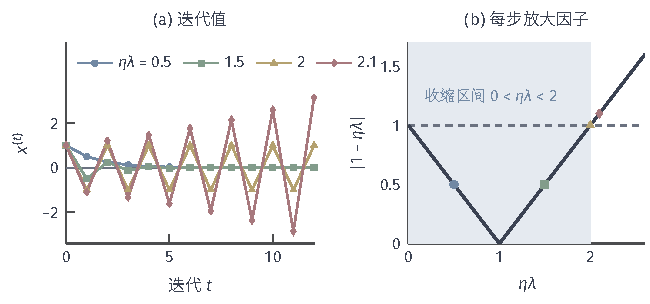
\includegraphics[width=110.0mm]{figures/03-optimization-evolution-and-signals/01-optimization/tikz/c3-step-size/figure.pdf}
  \caption{一维二次目标$f(x)=\lambda x^2/2$上的固定步长梯度下降，$x^{(0)}=1$。(a) 迭代值$x^{(t)}=(1-\eta\lambda)^t$，图例给出$\eta\lambda$；点只对应整数步，连线帮助追踪次序。(b) 每步的放大因子$|1-\eta\lambda|$，浅蓝区间$0<\eta\lambda<2$内因子小于$1$，四个彩色点对应(a)中的四个步长。}
  \label{fig:opt-smooth-step-size}
\end{figure}

\paragraph{共同例中的“之”字路径}
在二维共同例~\eqref{eq:opt-smooth-common-quadratic}上，两个坐标各自独立地按一维规律演化：$x_1$每步乘$1-\eta$，$x_2$每步乘$1-16\eta$。稳定要求$\eta<2/16=1/8$，由陡的$x_2$方向决定；而收敛快慢由最慢的因子决定。图~\ref{fig:opt-smooth-gd-zigzag}比较了三个步长。$\eta=1/16$时$x_2$一步归零，此后$x_1$每步只缩小到$15/16$；$\eta=2/17$使两个因子的绝对值相等，都是$15/17\approx0.882$，这是固定步长下的最佳折中，但$x_2$每步换号，路径在谷底两侧来回折返；$\eta=0.13$略超过$1/8$，$x_2$的因子为$-1.08$，路径越来越宽地横跨山谷，虽然$x_1$仍在收缩。一般地，对特征值在$[\mu,L]$中的正定二次目标，固定步长的最小最坏收缩因子是$(\kappa-1)/(\kappa+1)$，在$\eta=2/(L+\mu)$时取得；$\kappa$越大，路径越接近直线往返，收敛越慢。

\begin{figure*}[htbp]
  \centering
  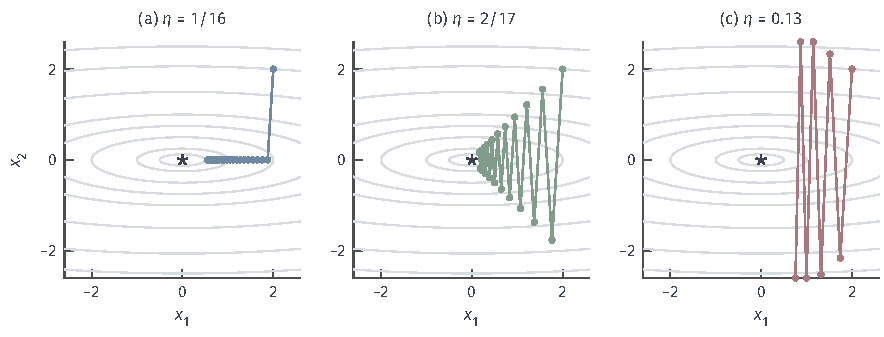
\includegraphics[width=149.7mm]{figures/03-optimization-evolution-and-signals/01-optimization/tikz/c3-gd-zigzag/figure.pdf}
  \caption{共同例$f(\bm x)=\tfrac12(x_1^2+16x_2^2)$上从$(2,2)^\top$出发的梯度下降路径，灰色椭圆是等高线，星号是最小点。(a) $\eta=1/16$：$x_2$一步消去，此后沿$x_1$轴缓慢前进（20步后$f\approx0.15$）。(b) $\eta=2/17$：两坐标因子为$\pm15/17$，路径呈“之”字。(c) $\eta=0.13>1/8$：$x_2$的因子为$-1.08$，路径越摆越宽（超出画面的点截在边框上）。}
  \label{fig:opt-smooth-gd-zigzag}
\end{figure*}

\paragraph{凸目标上的目标差}
若目标还是凸的，并且存在最小点，就可以从驻点残差推进到目标差。关键是把目标差和到最小点的距离联系起来。

\begin{theorem}[凸光滑目标上的梯度下降]
\label{thm:opt-smooth-gd-convex}
设$f$在$\mathbb R^d$上凸且$L$光滑，存在最小点$\bm x^\star$，取$\eta=1/L$。则对$T\geq1$，
\begin{equation}
\label{eq:opt-smooth-gd-convex-rate}
  f(\bm x^{(T)})-f^\star\leq\frac{L\lVert\bm x^{(0)}-\bm x^\star\rVert_2^2}{2T}.
\end{equation}
\end{theorem}

\begin{proof}
记$\bm g=\nabla f(\bm x)$，$\bm x^+=\bm x-\bm g/L$。由式~\eqref{eq:opt-smooth-gd-one-step}，$f(\bm x^+)\leq f(\bm x)-\lVert\bm g\rVert_2^2/(2L)$；由第~\ref{chap:optimization}章可微凸函数的一阶支撑下界，$f(\bm x)\leq f^\star+\langle\bm g,\bm x-\bm x^\star\rangle$。两式相加，再配方：
\[
  \begin{aligned}
  f(\bm x^+)-f^\star&\leq\langle\bm g,\bm x-\bm x^\star\rangle-\frac1{2L}\lVert\bm g\rVert_2^2\\
  &=\frac L2\Bigl(\lVert\bm x-\bm x^\star\rVert_2^2-\bigl\lVert\bm x-\bm x^\star-\tfrac1L\bm g\bigr\rVert_2^2\Bigr)\\
  &=\frac L2\bigl(\lVert\bm x-\bm x^\star\rVert_2^2-\lVert\bm x^+-\bm x^\star\rVert_2^2\bigr).
  \end{aligned}
\]
对$t=0,\dots,T-1$相加，右边相消为$\tfrac L2(\lVert\bm x^{(0)}-\bm x^\star\rVert_2^2-\lVert\bm x^{(T)}-\bm x^\star\rVert_2^2)\leq\tfrac L2\lVert\bm x^{(0)}-\bm x^\star\rVert_2^2$。左边是$\sum_{t=1}^{T}(f(\bm x^{(t)})-f^\star)$；目标值逐步不增，所以这个和不小于$T(f(\bm x^{(T)})-f^\star)$。
\end{proof}

证明顺带说明$\lVert\bm x^{(t)}-\bm x^\star\rVert_2$逐步不增：迭代点不会远离任何一个最小点。这个结论用到凸性；没有凸性时只有定理~\ref{thm:opt-smooth-gd-nonconvex}的残差保证。

\paragraph{回溯线搜索}
固定步长要求事先知道$L$。估计偏大则步长过小、进展缓慢；估计偏小则式~\eqref{eq:opt-smooth-gd-one-step}的系数可能为负，下降保证失效。另一种做法是不预先相信任何常数，而用实际函数值检验每一步：先试一个较大的步长，若目标没有“足够地”下降就缩小，直到下降为止。这里“足够”是指实际下降至少达到一阶预测的固定比例。设$\bm g\neq\bm0$，参数$c\in(0,1)$，\term{Armijo条件}（Armijo condition）要求
\begin{equation}
\label{eq:opt-smooth-armijo}
  f(\bm x-\eta\bm g)\leq f(\bm x)-c\,\eta\lVert\bm g\rVert_2^2 .
\end{equation}
右边是把切线的斜率打了折扣$c$的直线。按固定比例缩小步长直到满足它，称为\term{回溯线搜索}（backtracking line search），它是\term{线搜索}（line search）最常用的形式。

\begin{algorithm}[带回溯线搜索的一步梯度下降]
\label{alg:opt-smooth-backtracking}
\begin{algorithmic}[1]
\Require 当前点$\bm x$与梯度$\bm g=\nabla f(\bm x)\neq\bm0$，函数值$f(\bm x)$，初始试探步长$\bar\eta>0$，缩减比例$\gamma\in(0,1)$，参数$c\in(0,1)$
\Ensure 接受的步长$\eta$与新点$\bm x^+$
\State $\eta\gets\bar\eta$
\State 计算试探点$\bm x-\eta\bm g$的函数值
\While{$f(\bm x-\eta\bm g)>f(\bm x)-c\eta\lVert\bm g\rVert_2^2$}
  \State $\eta\gets\gamma\eta$ \Comment{拒绝试探点，缩短步长}
  \State 计算新试探点的函数值
\EndWhile
\State \Return $\eta$，$\bm x^+=\bm x-\eta\bm g$
\end{algorithmic}
\end{algorithm}

执行次序是：先算试探点的函数值，与右边的阈值比较；不满足就丢弃该点、缩短步长，再算下一个试探点。每次拒绝多花一次函数值计算，不需要新的梯度。若$\bm g=\bm0$，算法在线搜索之前已按驻点停止。

\begin{example}[共同例上的一次回溯]
\label{ex:opt-smooth-armijo}
在$\bm x^{(0)}=(2,2)^\top$处，$\bm g=(2,32)^\top$，$\lVert\bm g\rVert_2^2=1028$。取$\bar\eta=1$，$\gamma=1/2$，$c=1/4$，阈值为$34-257\eta$。依次试探：$\eta=1$时$f=7200$；$\eta=1/2$时$f=1568.5$；$\eta=1/4$时$f\approx289.1$；$\eta=1/8$时试探点为$(1.75,-2)^\top$，$f\approx33.53$，虽然低于$34$，却高于阈值$1.875$，仍被拒绝；$\eta=1/16$时试探点为$(1.875,0)^\top$，$f\approx1.758$，低于阈值$17.94$，接受。共计算了五次函数值、拒绝四次。图~\ref{fig:opt-smooth-armijo}画出最后两次试探：曲线$\varphi(\eta)=f(\bm x-\eta\bm g)$落在Armijo线下方的步长构成绿色区间。$\eta=1/8$被拒绝说明，“目标比原来低”还不够，Armijo条件要求下降与步长成比例。
\end{example}

\begin{figure}[htbp]
  \centering
  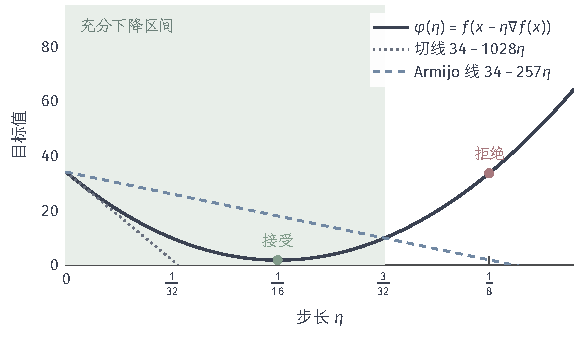
\includegraphics[width=98.0mm]{figures/03-optimization-evolution-and-signals/01-optimization/tikz/c3-armijo/figure.pdf}
  \caption{共同例在$\bm x=(2,2)^\top$处沿负梯度的一维截面$\varphi(\eta)=f(\bm x-\eta\nabla f(\bm x))$。点线是切线$34-1028\eta$，蓝色虚线是$c=1/4$的Armijo线$34-257\eta$，绿色区间是满足Armijo条件的步长。从$\bar\eta=1$开始减半，$\eta=1,\,1/2,\,1/4$的函数值远在画面之外，$\eta=1/8$（红点）虽使目标略降却在Armijo线之上被拒绝，$\eta=1/16$（绿点）被接受。}
  \label{fig:opt-smooth-armijo}
\end{figure}

\paragraph{回溯的有限结束与保证}
回溯的价值在于：它不需要知道$L$，但只要$L$存在，就一定有限步结束，且接受的步长不会太小。由式~\eqref{eq:opt-smooth-gd-one-step}，$\eta\leq2(1-c)/L$时$1-L\eta/2\geq c$，Armijo条件必然成立。因此当$f$为$L$光滑时，试探步长一旦落到$2(1-c)/L$以下就被接受，至多拒绝$\lceil\log_{1/\gamma}(\bar\eta L/(2(1-c)))\rceil$次（$\bar\eta\leq2(1-c)/L$时不拒绝），接受的步长满足
\[
  \eta\geq\eta_{\min}=\min\Bigl\{\bar\eta,\ \frac{2\gamma(1-c)}{L}\Bigr\}.
\]
例~\ref{ex:opt-smooth-armijo}中$2(1-c)/L=3/32$，实际接受的$1/16$确实不小于$\gamma\cdot3/32$。

每步下降至少$c\,\eta_{\min}\lVert\bm g^{(t)}\rVert_2^2$，按定理~\ref{thm:opt-smooth-gd-nonconvex}的证明累加，非凸情形得到$\min_{t<T}\lVert\nabla f(\bm x^{(t)})\rVert_2^2\leq(f(\bm x^{(0)})-f_{\inf})/(Tc\,\eta_{\min})$。凸情形若取$c=1/2$，接受的步长$\eta^{(t)}$满足$f(\bm x^{(t+1)})\leq f(\bm x^{(t)})-\tfrac{\eta^{(t)}}2\lVert\bm g^{(t)}\rVert_2^2$；把定理~\ref{thm:opt-smooth-gd-convex}证明中的$1/L$换成$\eta^{(t)}$，同样的配方给出
\[
  \eta^{(t)}\bigl(f(\bm x^{(t+1)})-f^\star\bigr)\leq\frac12\bigl(\lVert\bm x^{(t)}-\bm x^\star\rVert_2^2-\lVert\bm x^{(t+1)}-\bm x^\star\rVert_2^2\bigr),
\]
相加并利用目标单调与$\eta^{(t)}\geq\eta_{\min}$，得到$f(\bm x^{(T)})-f^\star\leq\lVert\bm x^{(0)}-\bm x^\star\rVert_2^2/(2T\eta_{\min})$，这里$\eta_{\min}=\min\{\bar\eta,\gamma/L\}$。这两条保证分别针对历史最佳残差点和最后一点，与固定步长的情形一致。回溯的代价是每轮多出的函数值计算；它不能弥补错误的梯度，也不能处理无下界的目标。

\subsection{预条件与坐标变换}
\label{sec:opt-smooth-preconditioning}

“之”字路径的根源是同一个标量步长要同时服务于曲率$1$和曲率$16$两个方向。若能对不同方向使用不同的步长，例如$x_1$方向走$1$、$x_2$方向走$1/16$，一步就能到达原点。本小节把这种想法写成固定的线性坐标变换。

\paragraph{固定预条件就是换坐标}
取固定的对称正定矩阵$\bm P$，更新
\begin{equation}
\label{eq:opt-smooth-preconditioned-gd}
  \bm x^{(t+1)}=\bm x^{(t)}-\eta\bm P\nabla f(\bm x^{(t)})
\end{equation}
称为\term{预条件}（preconditioning）梯度法，$\bm P$称为预条件矩阵。令$\bm x=\bm P^{1/2}\bm z$，定义$h(\bm z)=f(\bm P^{1/2}\bm z)$。由链式法则$\nabla h(\bm z)=\bm P^{1/2}\nabla f(\bm x)$，对$h$作普通梯度下降$\bm z^+=\bm z-\eta\nabla h(\bm z)$，两边左乘$\bm P^{1/2}$恰好得到式~\eqref{eq:opt-smooth-preconditioned-gd}。所以预条件梯度法就是在新坐标$\bm z$中的普通梯度下降：它不改变目标的值和最小点，只改变“哪个方向算作一步”。新坐标中的Hessian是
\[
  \nabla^2h(\bm z)=\bm P^{1/2}\,\nabla^2f(\bm x)\,\bm P^{1/2},
\]
它与$\bm P\nabla^2f(\bm x)$相似，因而特征值相同。对正定二次目标$\tfrac12\bm x^\top\bm H\bm x$，上一小节的全部结论在$\bm z$坐标中成立：收敛当且仅当$0<\eta<2/\lambda_{\max}(\bm P^{1/2}\bm H\bm P^{1/2})$，最佳固定步长的收缩因子为$(\tilde\kappa-1)/(\tilde\kappa+1)$，其中$\tilde\kappa$是变换后Hessian的条件数。

\begin{example}[共同例上的两个预条件]
\label{ex:opt-smooth-preconditioning}
取$\bm P=\operatorname{diag}(1,1/16)$，则$\bm P\nabla f(\bm x)=\bm x$，变换后Hessian为$\bm I$，$\tilde\kappa=1$。取$\eta=1/2$，每步$\bm x^{(t+1)}=\bm x^{(t)}/2$，迭代沿对角线直奔原点；取$\eta=1$则一步到达。反过来取$\bm P=\operatorname{diag}(1/16,1)$，它的条件数同样是$16$，变换后Hessian却是$\operatorname{diag}(1/16,16)$，条件数$256$，最佳固定步长的收缩因子从$15/17\approx0.882$恶化到$255/257\approx0.992$。图~\ref{fig:opt-smooth-preconditioning}在三个坐标系中画出这三种情形：在合适的$\bm z$坐标中，椭圆等高线变成圆，负梯度直接指向圆心；在不合适的坐标中，椭圆反而被拉得更扁。
\end{example}

\begin{figure*}[htbp]
  \centering
  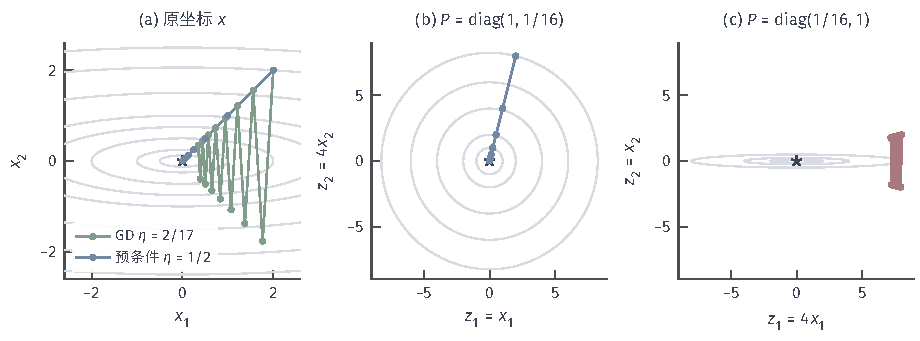
\includegraphics[width=155.7mm]{figures/03-optimization-evolution-and-signals/01-optimization/tikz/c3-preconditioning/figure.pdf}
  \caption{固定预条件作为坐标变换。(a) 原坐标中，普通梯度下降（绿，$\eta=2/17$）走“之”字，$\bm P=\operatorname{diag}(1,1/16)$、$\eta=1/2$的预条件更新（蓝）每步把$\bm x$减半，沿直线到达原点。(b) 在$\bm z=\bm P^{-1/2}\bm x=(x_1,4x_2)$坐标中，等高线是圆，蓝色路径就是普通梯度下降。(c) 若取$\bm P=\operatorname{diag}(1/16,1)$，$\bm z=(4x_1,x_2)$，变换后Hessian为$\operatorname{diag}(1/16,16)$，等高线更扁；红色是此坐标中最佳固定步长$\eta=2/(16+1/16)$的14步，每步横跨山谷，沿长轴几乎不动。}
  \label{fig:opt-smooth-preconditioning}
\end{figure*}

例子说明，判断预条件好坏的标准是变换后的曲率$\bm P^{1/2}\bm H\bm P^{1/2}$，而不是$\bm P$自身的条件数。理想的$\bm P$是$\bm H^{-1}$，但求它等于解原问题；实际的预条件在“变换后曲率接近常数倍单位阵”与“构造和应用$\bm P$的成本”之间折中。对角$\bm P$每轮只多$O(d)$次乘法，稠密$\bm P$需要$O(d^2)$存储与每轮$O(d^2)$运算，若$\bm P$以分解形式给出，成本取决于分解结构。本小节的分析要求$\bm P$在迭代中固定；按历史梯度统计逐轮改变的缩放，其构造、正定性与收敛分析在第~\ref{chap:opt-stochastic-block}章讨论。

\paragraph{选定度量中的最陡下降}
预条件还有另一种读法：它改变了“最陡”的含义。给定对称正定矩阵$\bm M$，定义范数$\lVert\bm v\rVert_{\bm M}=\sqrt{\bm v^\top\bm M\bm v}$。在单位$\bm M$-球上使方向导数最小的方向，称为该度量下的\term{最陡下降方向}（steepest descent direction）。由$\bm M$-内积的Cauchy--Schwarz不等式，
\[
  \langle\bm g,\bm d\rangle=(\bm M^{-1}\bm g)^\top\bm M\bm d\geq-\lVert\bm M^{-1}\bm g\rVert_{\bm M}\lVert\bm d\rVert_{\bm M},
\]
等号在$\bm d$与$-\bm M^{-1}\bm g$同向时取得，所以最陡下降方向是$-\bm M^{-1}\bm g/\lVert\bm M^{-1}\bm g\rVert_{\bm M}$。取$\bm M=\bm I$得到负梯度，取$\bm M=\bm P^{-1}$得到$-\bm P\bm g$的方向。负梯度只是欧氏度量下的最陡方向；同一个目标在不同度量下有不同的“最陡”方向。

换了度量，与之配套的光滑常数和残差也要一起换。若对所有$\bm x,\bm p$有$f(\bm x+\bm p)\leq f(\bm x)+\langle\bm g,\bm p\rangle+\tfrac{L_{\bm M}}2\lVert\bm p\rVert_{\bm M}^2$，把$\bm p=-\eta\bm M^{-1}\bm g$代入，与式~\eqref{eq:opt-smooth-gd-one-step}同样的推导给出
\[
  f(\bm x^+)\leq f(\bm x)-\eta\Bigl(1-\frac{L_{\bm M}\eta}2\Bigr)\bm g^\top\bm M^{-1}\bm g .
\]
步长上限由$L_{\bm M}$决定，衡量进展的残差是$\sqrt{\bm g^\top\bm M^{-1}\bm g}$，而不再是$\lVert\bm g\rVert_2$。共同例取$\bm M=\operatorname{diag}(1,16)$时$L_{\bm M}=1$，残差$\sqrt{g_1^2+g_2^2/16}$；用欧氏残差$\lVert\bm g\rVert_2$作停止判据，同样的容差在两个坐标方向上就对应了相差$16$倍的精度要求。本章只用固定的正定度量；由概率模型诱导的Fisher度量与自然梯度属于分布几何，可参考\BookChapterRef{chap:information-theory-and-statistical-geometry}{卷四“概率分布的分析与优化”章}。

\subsection{重球动量法}
\label{sec:opt-smooth-heavy-ball}

预条件需要事先知道各方向的曲率。另一种思路不改坐标，而让更新记住前一步的位移。观察图~\ref{fig:opt-smooth-gd-zigzag}(b)：连续两步在$x_2$方向上符号相反，在$x_1$方向上符号相同。若把上一步的位移按比例叠加到这一步，横跨山谷的分量相互抵消，沿谷底的分量逐步累积，就像一个有惯性的小球沿槽滚下，而不是每步都重新起跑。

\paragraph{状态与一轮更新}
\term{重球法}（heavy-ball method）是经典的\term{动量法}（momentum method）\cite{polyak1964heavyball}，它的更新为
\begin{equation}
\label{eq:opt-smooth-heavy-ball}
  \bm x^{(t+1)}=\bm x^{(t)}-\eta\nabla f(\bm x^{(t)})+\beta\bigl(\bm x^{(t)}-\bm x^{(t-1)}\bigr),\qquad 0\leq\beta<1 .
\end{equation}
算法的完整状态是一对点$(\bm x^{(t)},\bm x^{(t-1)})$，等价地是当前点与上一步位移；只知道$\bm x^{(t)}$无法继续迭代。约定$\bm x^{(-1)}=\bm x^{(0)}$，即零动量启动，第一步就是普通梯度步。每轮仍只算一次梯度，额外的代价是存储一个向量和几次向量加法。$\beta=0$时退回梯度下降。

\paragraph{二次目标上的逐方向递推}
在正定二次目标$f(\bm x)=\tfrac12(\bm x-\bm x^\star)^\top\bm H(\bm x-\bm x^\star)$上，误差$\bm e^{(t)}=\bm x^{(t)}-\bm x^\star$满足$\bm e^{(t+1)}=(\bm I-\eta\bm H)\bm e^{(t)}+\beta(\bm e^{(t)}-\bm e^{(t-1)})$。在$\bm H$的特征向量基下各分量互不耦合，曲率为$\lambda$的分量满足二阶线性递推
\begin{equation}
\label{eq:opt-smooth-hb-recursion}
  e^{(t+1)}=(1+\beta-\eta\lambda)\,e^{(t)}-\beta\,e^{(t-1)} .
\end{equation}
它的解是特征方程$r^2-(1+\beta-\eta\lambda)r+\beta=0$两根的幂的组合（重根时还有$t\,r^t$项），所以收敛快慢由较大的根模决定。与梯度下降的一阶递推$e^{(t+1)}=(1-\eta\lambda)e^{(t)}$相比，多出的一项$-\beta e^{(t-1)}$使误差能以阻尼振荡的方式衰减：两根为共轭复数时，模都等于$\sqrt\beta$，与$\lambda$无关。

\paragraph{稳定范围与参数选择}
两根都在单位圆内的条件，可以由二次多项式$r^2+a_1r+a_0$的判据$|a_0|<1$、$|a_1|<1+a_0$读出：这里$a_0=\beta$、$a_1=-(1+\beta-\eta\lambda)$，条件化为
\[
  0<\eta\lambda<2(1+\beta).
\]
动量把稳定的步长上界从$2/L$放宽到$2(1+\beta)/L$。根为复数当且仅当$(1+\beta-\eta\lambda)^2<4\beta$，即$(1-\sqrt\beta)^2<\eta\lambda<(1+\sqrt\beta)^2$，此时根模恰为$\sqrt\beta$。若谱区间$[\mu,L]$已知，选$\eta,\beta$使$\eta\mu=(1-\sqrt\beta)^2$、$\eta L=(1+\sqrt\beta)^2$，整个区间都落在复根区（端点为重根），解得
\begin{equation}
\label{eq:opt-smooth-hb-parameters}
  \eta=\frac{4}{(\sqrt L+\sqrt\mu)^2},\qquad
  \beta=\Bigl(\frac{\sqrt L-\sqrt\mu}{\sqrt L+\sqrt\mu}\Bigr)^2,\qquad
  \sqrt\beta=\frac{\sqrt\kappa-1}{\sqrt\kappa+1}.
\end{equation}
每个方向的根模都不超过$\sqrt\beta$，端点处重根带来的$t\,r^t$因子只使衰减慢一个多项式倍数。共同例中$\kappa=16$，得$\eta=4/25$、$\beta=9/25$、$\sqrt\beta=3/5$，而梯度下降的最佳因子是$15/17\approx0.882$。达到同一误差所需的轮数大约正比于$1/(1-\text{因子})$，前者约$\sqrt\kappa/2$、后者约$\kappa/2$，这就是“加速”一词的含义。

图~\ref{fig:opt-smooth-momentum-stability}画出最大根模随$\eta\lambda$的变化。$\beta=9/25$的曲线在浅蓝区间$[\eta\mu,\eta L]=[0.16,2.56]$上平坦地等于$0.6$；$\beta=0$即梯度下降，曲线是折线$|1-\eta\lambda|$，只在$\eta\lambda=1$附近较低；$\beta=0.81$的稳定范围更宽（到$3.62$），平坦部分却抬高到$0.9$。动量过大并不会立即发散，而是让误差以接近$1$的模长期振荡；$\eta\lambda$超过$2(1+\beta)$时则一定发散。

\begin{figure}[htbp]
  \centering
  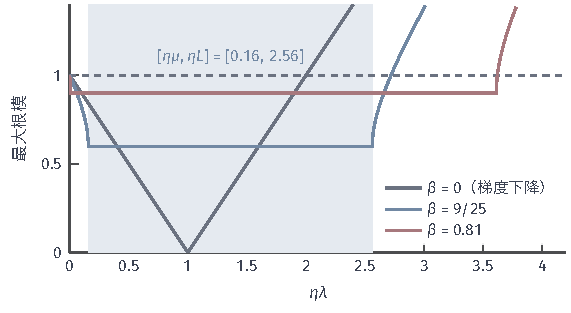
\includegraphics[width=96.6mm]{figures/03-optimization-evolution-and-signals/01-optimization/tikz/c3-momentum-stability/figure.pdf}
  \caption{重球法递推~\eqref{eq:opt-smooth-hb-recursion}的最大根模与$\eta\lambda$的关系（大于$1.4$的部分截去）。灰线$\beta=0$即梯度下降；蓝线$\beta=9/25$对应共同例的参数~\eqref{eq:opt-smooth-hb-parameters}，在浅蓝区间$[\eta\mu,\eta L]=[0.16,2.56]$上恒为$0.6$；红线$\beta=0.81$在复根区恒为$0.9$。虚线是稳定边界$1$。}
  \label{fig:opt-smooth-momentum-stability}
\end{figure}

\paragraph{结论的范围}
动量使目标值不再逐步单调。在共同例上用参数~\eqref{eq:opt-smooth-hb-parameters}，第一步是步长$4/25$的普通梯度步，这个步长超过了梯度下降的稳定上界$1/8$：$\bm x^{(1)}=(1.68,-3.12)^\top$，目标从$34$升到约$79.29$；此后惯性项开始抵消横向摆动，图~\ref{fig:opt-smooth-momentum-paths}中的蓝色曲线在第$10$步前后降到梯度下降之下。以上稳定范围和速率都是在正定二次目标、已知谱界的条件下逐方向算出的。对一般强凸光滑目标，重球法用这组参数并不保证全局收敛；对非凸目标，二次例的加速结论更不能直接继承。实际使用动量时，停止判据仍应检查原目标的梯度范数，而不是位移或动量的大小。

\subsection{Nesterov加速梯度法}
\label{sec:opt-smooth-nesterov}

重球法在当前点求梯度，再叠加惯性；它的加速分析依赖二次目标的逐方向分解。Nesterov提出的做法改变了求梯度的位置：先沿惯性方向外推到一个前瞻点，在那里求梯度并走一步。这一改动使加速结论能够推广到一般的凸光滑目标\cite{nesterov1983method}。

\paragraph{三个点与一轮更新}
\term{Nesterov加速梯度}（Nesterov accelerated gradient）区分三类点：记录点$\bm x^{(t)}$，外推得到的前瞻点$\bm y^{(t)}$，以及在$\bm y^{(t)}$处求得的梯度。下面是凸、$L$光滑目标的一个版本\cite{beck2009fista}。

\begin{algorithm}[Nesterov加速梯度法]
\label{alg:opt-smooth-nesterov}
\begin{algorithmic}[1]
\Require $L$光滑凸目标$f$，常数$L$，初值$\bm x^{(0)}$，轮数$T$
\Ensure 最后一点$\bm x^{(T)}$
\State $\bm y^{(0)}\gets\bm x^{(0)}$，$\theta^{(0)}\gets1$
\For{$t=0,1,\dots,T-1$}
  \State $\bm x^{(t+1)}\gets\bm y^{(t)}-\frac1L\nabla f(\bm y^{(t)})$ \Comment{在前瞻点求梯度}
  \State $\theta^{(t+1)}\gets\bigl(1+\sqrt{1+4(\theta^{(t)})^2}\bigr)/2$
  \State $\bm y^{(t+1)}\gets\bm x^{(t+1)}+\dfrac{\theta^{(t)}-1}{\theta^{(t+1)}}\bigl(\bm x^{(t+1)}-\bm x^{(t)}\bigr)$ \Comment{外推}
\EndFor
\end{algorithmic}
\end{algorithm}

把更新写成与重球法相同的形状，记$\beta^{(t)}=(\theta^{(t-1)}-1)/\theta^{(t)}$（$t\geq1$，$\beta^{(0)}=0$），则
\[
  \text{重球法：}\ \bm x^{(t+1)}=\bm x^{(t)}+\beta(\bm x^{(t)}-\bm x^{(t-1)})-\eta\nabla f(\bm x^{(t)}),
\]
\[
  \text{Nesterov：}\ \bm x^{(t+1)}=\bm x^{(t)}+\beta^{(t)}(\bm x^{(t)}-\bm x^{(t-1)})-\tfrac1L\nabla f\bigl(\bm x^{(t)}+\beta^{(t)}(\bm x^{(t)}-\bm x^{(t-1)})\bigr).
\]
两者都把惯性项加到当前点上，区别只在梯度的求值位置：重球法在出发点求，Nesterov在惯性已经带到的位置求。若惯性把点带过了谷底，前瞻点处的梯度会把它拉回来，这是一种“提前修正”。另一个区别是$\beta^{(t)}$随$t$增大而趋于$1$，不需要知道$\mu$。每轮的代价仍是一次梯度和几次向量运算，状态是$(\bm x^{(t)},\bm x^{(t-1)},\theta^{(t)})$。

\paragraph{加速保证}
在凸、光滑、最小点存在的条件下，Nesterov方法的目标差以$1/T^2$的速度下降，而定理~\ref{thm:opt-smooth-gd-convex}给出的梯度下降保证是$1/T$。证明不比较相邻两步的目标值，而是构造一个把目标差与距离合在一起的量，即\term{势函数}（potential function），证明它逐步不增。

\begin{theorem}[Nesterov方法的收敛速度]
\label{thm:opt-smooth-nesterov}
设$f$在$\mathbb R^d$上凸且$L$光滑（$L>0$），存在最小点$\bm x^\star$。则算法~\ref{alg:opt-smooth-nesterov}的迭代满足
\begin{equation}
\label{eq:opt-smooth-nesterov-rate}
  f(\bm x^{(T)})-f^\star\leq\frac{2L\lVert\bm x^{(0)}-\bm x^\star\rVert_2^2}{(T+1)^2},\qquad T\geq1 .
\end{equation}
\end{theorem}

\begin{proof}
\emph{三点不等式。}对任意$\bm y$，令$\bm x^+=\bm y-\nabla f(\bm y)/L$。下降引理给$f(\bm x^+)\leq f(\bm y)-\lVert\nabla f(\bm y)\rVert_2^2/(2L)$，凸性给$f(\bm y)\leq f(\bm v)+\langle\nabla f(\bm y),\bm y-\bm v\rangle$对任意$\bm v$成立。相加后与定理~\ref{thm:opt-smooth-gd-convex}的证明一样配方，得
\begin{equation}
\label{eq:opt-smooth-three-point}
  f(\bm x^+)\leq f(\bm v)+\frac L2\bigl(\lVert\bm y-\bm v\rVert_2^2-\lVert\bm x^+-\bm v\rVert_2^2\bigr).
\end{equation}

\emph{选比较点。}记$\Delta^{(t)}=f(\bm x^{(t)})-f^\star$，$\theta=\theta^{(t)}$。在式~\eqref{eq:opt-smooth-three-point}中取$\bm y=\bm y^{(t)}$，$\bm v=(1-1/\theta)\bm x^{(t)}+\bm x^\star/\theta$。由$\theta\geq1$，$\bm v$是$\bm x^{(t)}$与$\bm x^\star$的凸组合，凸性给$f(\bm v)-f^\star\leq(1-1/\theta)\Delta^{(t)}$。引入辅助点$\bm u^{(t)}=\theta^{(t)}\bm y^{(t)}-(\theta^{(t)}-1)\bm x^{(t)}$，直接展开可得$\bm y^{(t)}-\bm v=(\bm u^{(t)}-\bm x^\star)/\theta$，以及$\bm x^{(t+1)}-\bm v=\bigl(\theta\bm x^{(t+1)}-(\theta-1)\bm x^{(t)}-\bm x^\star\bigr)/\theta$。把外推公式代入$\bm u^{(t+1)}$的定义：
\[
  \begin{aligned}
  \bm u^{(t+1)}&=\theta^{(t+1)}\bm x^{(t+1)}+(\theta^{(t)}-1)(\bm x^{(t+1)}-\bm x^{(t)})-(\theta^{(t+1)}-1)\bm x^{(t+1)}\\
  &=\theta^{(t)}\bm x^{(t+1)}-(\theta^{(t)}-1)\bm x^{(t)},
  \end{aligned}
\]
所以$\bm x^{(t+1)}-\bm v=(\bm u^{(t+1)}-\bm x^\star)/\theta$。于是式~\eqref{eq:opt-smooth-three-point}变为
\[
  \Delta^{(t+1)}\leq\Bigl(1-\frac1{\theta^{(t)}}\Bigr)\Delta^{(t)}+\frac{L}{2(\theta^{(t)})^2}\bigl(\lVert\bm u^{(t)}-\bm x^\star\rVert_2^2-\lVert\bm u^{(t+1)}-\bm x^\star\rVert_2^2\bigr).
\]

\emph{势函数不增。}两边乘$(\theta^{(t)})^2$。参数的更新式等价于$(\theta^{(t)})^2-\theta^{(t)}=(\theta^{(t-1)})^2$（$t\geq1$），而$\theta^{(0)}=1$使$(\theta^{(0)})^2-\theta^{(0)}=0$。定义势函数
\[
  E^{(0)}=\frac L2\lVert\bm x^{(0)}-\bm x^\star\rVert_2^2,\qquad
  E^{(t)}=(\theta^{(t-1)})^2\Delta^{(t)}+\frac L2\lVert\bm u^{(t)}-\bm x^\star\rVert_2^2\quad(t\geq1),
\]
注意$\bm u^{(0)}=\bm x^{(0)}$，上式正是$E^{(t+1)}\leq E^{(t)}$，对所有$t\geq0$成立。因此$(\theta^{(T-1)})^2\Delta^{(T)}\leq E^{(T)}\leq E^{(0)}$。

\emph{参数的增长。}由$\theta^{(t+1)}=\bigl(1+\sqrt{1+4(\theta^{(t)})^2}\bigr)/2\geq(1+2\theta^{(t)})/2=\theta^{(t)}+1/2$及$\theta^{(0)}=1$，归纳得$\theta^{(t)}\geq(t+2)/2$。取$t=T-1$代入上一段即得式~\eqref{eq:opt-smooth-nesterov-rate}。
\end{proof}

证明中下降的是势函数$E^{(t)}$，而不是目标值本身。势函数的第二项会随迭代把“能量”转给第一项，所以目标值可以在某些步上升。图~\ref{fig:opt-smooth-momentum-paths}(b)中，Nesterov方法的目标差在共同例上呈阶梯状起伏，但始终位于绿色点线所示的上界$2L\lVert\bm x^{(0)}-\bm x^\star\rVert_2^2/(t+1)^2=256/(t+1)^2$之下。

\begin{figure*}[htbp]
  \centering
  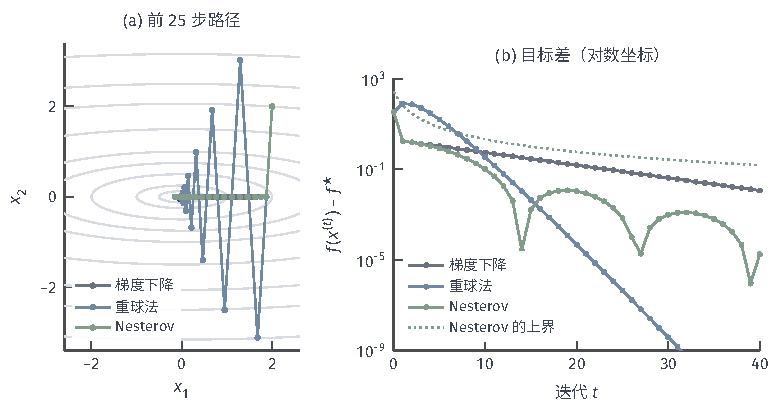
\includegraphics[width=132.0mm]{figures/03-optimization-evolution-and-signals/01-optimization/tikz/c3-momentum-paths/figure.pdf}
  \caption{共同例上梯度下降（灰，$\eta=1/16$）、重球法（蓝，$\eta=4/25$、$\beta=9/25$）与Nesterov方法（绿，$L=16$）的比较，均从$(2,2)^\top$出发、每轮一次梯度。(a) 前25步的路径；重球法第一步越到$(1.68,-3.12)^\top$，随后惯性抵消横向摆动。(b) 目标差的对数坐标曲线：重球法按约$0.6^{2t}$下降，梯度下降按$(15/16)^{2t}$下降，Nesterov方法的曲线不单调，但始终在点线所示的$O(1/t^2)$上界之下。}
  \label{fig:opt-smooth-momentum-paths}
\end{figure*}

\paragraph{使用时的边界}
共同例是强凸的，图中重球法用了已知的$\mu$而快于Nesterov方法的凸版本；若同样已知$\mu$，Nesterov方法也有常数动量$(\sqrt\kappa-1)/(\sqrt\kappa+1)$的强凸版本，这里不展开。定理~\ref{thm:opt-smooth-nesterov}要求精确梯度、步长$1/L$与凸性；$L$未知时，回溯必须与加速方案的势函数配套设计，不能把算法~\ref{alg:opt-smooth-backtracking}直接套上。实现中常加入\emph{重启}：当目标值上升或动量方向与梯度夹角变钝时，把$\theta$重置为$1$，以抑制振荡。重启是经验上有效的补充，在凸情形下并不改变定理的结论；对非凸目标，加速的速率保证不能无条件搬用，仍须以原目标的梯度残差作停止判据。

\section{曲率与局部模型}
\label{sec:opt-smooth-local-models}

梯度方法用一个统一的$L$代替所有方向的曲率，预条件和动量只是在不知道真实曲率时的补救。若能读取二阶导数，就可以在当前点用二次模型~\eqref{eq:opt-smooth-quadratic-model}更贴切地代替目标，取$\bm B$为真实或近似的Hessian。这样做会遇到四个问题，本节按它们组织：曲率从哪里来（Hessian、修正后的Hessian，或由梯度差拼出的近似）；怎样保证模型可用（正定化、限制位移、加立方项）；怎样求解模型（直接分解或只用矩阵向量积的迭代）；以及怎样决定是否接受模型给出的位移（线搜索或比较实际与预测的下降）。贯穿始终的一点是：模型的最小点只是候选，原目标的检验不能省略；模型在局部最优，也不意味着原非凸目标已经全局最优。本节记$\bm g=\nabla f(\bm x)$，$\bm H=\nabla^2 f(\bm x)$；Hessian在某区域内的Lipschitz常数记为$M$，即$\lVert\nabla^2f(\bm u)-\nabla^2f(\bm v)\rVert_2\leq M\lVert\bm u-\bm v\rVert_2$。

\subsection{牛顿法}
\label{sec:opt-smooth-newton}

\paragraph{牛顿方程}
多元Taylor展开在$\bm x$附近给出二次模型
\[
  m(\bm p)=f(\bm x)+\langle\bm g,\bm p\rangle+\frac12\bm p^\top\bm H\bm p,
\]
其二阶余项的控制可参考\BookChapterRef{chap:multivariate-calculus}{卷一“多元函数微分”章}。令模型的梯度$\bm g+\bm H\bm p$为零，得到\term{牛顿法}（Newton's method）的方程与更新
\begin{equation}
\label{eq:opt-smooth-newton}
  \bm H\bm p^{\mathrm N}=-\bm g,\qquad \bm x^+=\bm x+\eta\,\bm p^{\mathrm N}.
\end{equation}
实际计算解这个线性方程，而不显式求$\bm H^{-1}$：$\bm H$正定时用Cholesky分解，稠密情形约需$d^3/3$次乘加和$O(d^2)$存储；求逆不但更贵，数值上也更不稳定。线性方程的直接解法及其误差分析可参考\BookChapterRef{chap:linear-equations-and-optimization}{卷一“线性方程与矩阵方程”章}。

\paragraph{可逆与正定的不同作用}
$\bm H$可逆只保证方程有唯一解，也就是模型有唯一驻点；$\bm H$正定才使这个驻点是模型的唯一最小点，并且$\langle\bm g,\bm p^{\mathrm N}\rangle=-\bm g^\top\bm H^{-1}\bm g<0$，即牛顿方向是下降方向。$\bm H$不定时，牛顿方向可能指向上坡。取$f(\bm x)=\tfrac12x_1^2+\tfrac14x_2^4-\tfrac12x_2^2$，它在$(0,\pm1)$处取最小值，原点是鞍点。在$\bm x=(0,0.2)^\top$处，$\bm g=(0,-0.192)^\top$，$\bm H=\operatorname{diag}(1,-0.88)$可逆但不定，牛顿方向$\bm p^{\mathrm N}=(0,-0.218)^\top$满足$\langle\bm g,\bm p^{\mathrm N}\rangle\approx0.042>0$。沿它走一整步到达$(0,-0.018)^\top$，目标从$-0.0196$升到约$-0.0002$，迭代被拉向鞍点。原因是二次模型在$x_2$方向开口向下，它的驻点是模型的最大点。

\paragraph{阻尼牛顿法}
远离最小点时，即使$\bm H$正定，二次模型也可能很不准确，整步会越过头。\term{阻尼牛顿法}（damped Newton method）保持牛顿方向不变，从$\eta=1$开始回溯，直到满足方向形式的Armijo条件
\[
  f(\bm x+\eta\bm p^{\mathrm N})\leq f(\bm x)+c\,\eta\langle\bm g,\bm p^{\mathrm N}\rangle,\qquad 0<c<\tfrac12 .
\]
它要求$\bm p^{\mathrm N}$是下降方向；对上坡方向，把步长缩得再小也只会使目标上升。单位步长必须最先试探且合格即接受，这一点在解附近至关重要：若永久固定$\eta<1$，在二次目标上误差每步只乘以$1-\eta$，快速局部收敛就丧失了。

\paragraph{局部二次收敛}
在非退化最小点附近，牛顿法以惊人的速度收敛。

\begin{theorem}[牛顿法的局部二次收敛]
\label{thm:opt-smooth-newton-local}
设$f$在球$\mathcal B=\{\bm x:\lVert\bm x-\bm x^\star\rVert_2<r\}$上二阶连续可微，$\nabla f(\bm x^\star)=\bm0$，并且在$\mathcal B$上$\nabla^2f\succeq\mu\bm I$（$\mu>0$）、Hessian是$M$-Lipschitz的。若$\bm x\in\mathcal B$，则单位牛顿步$\bm x^+=\bm x-\nabla^2f(\bm x)^{-1}\nabla f(\bm x)$满足
\begin{equation}
\label{eq:opt-smooth-newton-quadratic}
  \lVert\bm x^+-\bm x^\star\rVert_2\leq\frac{M}{2\mu}\lVert\bm x-\bm x^\star\rVert_2^2 .
\end{equation}
因此若$\lVert\bm x^{(0)}-\bm x^\star\rVert_2<\min\{r,2\mu/M\}$，全部迭代留在$\mathcal B$中，且$\tfrac{M}{2\mu}\lVert\bm x^{(t)}-\bm x^\star\rVert_2\leq\bigl(\tfrac{M}{2\mu}\lVert\bm x^{(0)}-\bm x^\star\rVert_2\bigr)^{2^t}$。
\end{theorem}

\begin{proof}
记$\bm e=\bm x-\bm x^\star$，$\bm H=\nabla^2f(\bm x)$。由于$\nabla f(\bm x^\star)=\bm0$，沿线段积分得$\nabla f(\bm x)=\int_0^1\nabla^2f(\bm x^\star+s\bm e)\bm e\,\mathrm ds$，于是
\[
  \bm x^+-\bm x^\star=\bm e-\bm H^{-1}\nabla f(\bm x)=\bm H^{-1}\int_0^1\bigl(\bm H-\nabla^2f(\bm x^\star+s\bm e)\bigr)\bm e\,\mathrm ds .
\]
$\lVert\bm H^{-1}\rVert_2\leq1/\mu$，被积项的范数不超过$M(1-s)\lVert\bm e\rVert_2^2$，积分得$\tfrac M2\lVert\bm e\rVert_2^2$，即式~\eqref{eq:opt-smooth-newton-quadratic}。若$\tfrac M{2\mu}\lVert\bm e\rVert_2<1$，则$\lVert\bm x^+-\bm x^\star\rVert_2<\lVert\bm e\rVert_2$，新点仍在$\mathcal B$中；记$a_t=\tfrac M{2\mu}\lVert\bm x^{(t)}-\bm x^\star\rVert_2$，式~\eqref{eq:opt-smooth-newton-quadratic}即$a_{t+1}\leq a_t^2$，归纳即得结论。
\end{proof}

误差满足$\lVert\bm e^{(t+1)}\rVert\leq C\lVert\bm e^{(t)}\rVert^2$的收敛称为\term{二次收敛}（quadratic convergence）：进入$a_t<1$的区域后，每步有效数字大约翻倍。图~\ref{fig:opt-smooth-newton-model}用一维例子$f(x)=e^x-2x$展示这一点，其最小点$x^\star=\ln2\approx0.6931$。从$x^{(0)}=1.5$出发，牛顿更新为$x^+=x-1+2e^{-x}$，误差依次约为$0.81$、$0.25$、$0.029$、$4.3\times10^{-4}$、$9.3\times10^{-8}$、$4.3\times10^{-15}$；比值$|e^{(t+1)}|/|e^{(t)}|^2$趋于$f'''(x^\star)/(2f''(x^\star))=1/2$。同一区间上$f''\leq e^{1.5}$，步长$e^{-1.5}$的梯度下降误差每步大约只乘以$1-2e^{-1.5}\approx0.55$。

\begin{figure}[htbp]
  \centering
  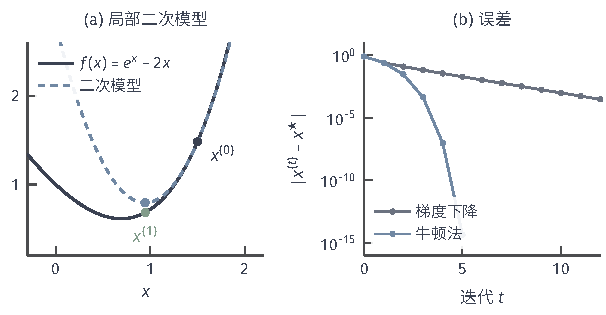
\includegraphics[width=102.6mm]{figures/03-optimization-evolution-and-signals/01-optimization/tikz/c3-newton-model/figure.pdf}
  \caption{牛顿法在$f(x)=e^x-2x$上的局部模型与误差。(a) 在$x^{(0)}=1.5$处的二阶Taylor模型（蓝色虚线）；它的最小点$x^{(1)}\approx0.946$就是牛顿步，模型值（蓝点）约$0.795$，真实目标（绿点）约$0.684$。(b) 误差$|x^{(t)}-\ln2|$的对数坐标：牛顿法（蓝）的曲线越来越陡，五步达到$10^{-15}$；步长$e^{-1.5}$的梯度下降（灰）是一条斜率固定的直线。}
  \label{fig:opt-smooth-newton-model}
\end{figure}

\paragraph{局部收敛阶与全程成本}
定理~\ref{thm:opt-smooth-newton-local}只描述已经进入半径$\min\{r,2\mu/M\}$的邻域之后的行为，这个邻域的大小在实际问题中通常未知。从远处出发时，阻尼牛顿法的线搜索阶段可能需要许多步，每步都要形成Hessian并分解，代价是$O(d^3)$；局部二次收敛只说明最后几步极快，不说明总成本低。两件事分开评价：局部收敛阶回答“到了附近以后误差怎样缩小”，全程成本回答“从初值到达给定精度一共做了多少工作”。第~\ref{sec:opt-smooth-accuracy-cost}节在共同标准下比较两者。

\subsection{修正牛顿法}
\label{sec:opt-smooth-modified-newton}

\paragraph{构造正定模型}
上一小节的例子说明，Hessian不定时牛顿方向可能上坡，而缩短步长无法补救：若$\langle\bm g,\bm p\rangle>0$，则对任意$\eta>0$都有$\langle\bm g,\eta\bm p\rangle>0$。补救必须改变方向本身。\term{修正牛顿法}（modified Newton method）把模型矩阵换成正定的$\bm B=\bm H+\bm E$，再解$\bm B\bm p=-\bm g$。最简单的修正是谱移位$\bm E=\delta\bm I$，取$\delta>\max\{0,-\lambda_{\min}(\bm H)\}$；不想计算特征值时，\term{修正Cholesky分解}（modified Cholesky factorization）在分解过程中遇到过小或负的主元就把它增大，同时得到某个正定的$\bm B$及其分解。在上一小节的点$(0,0.2)^\top$处取$\delta=1.88$，$\bm B=\operatorname{diag}(2.88,1)$，方向变为$(0,0.192)^\top$，沿它走一整步到$(0,0.392)^\top$，目标从$-0.0196$降到约$-0.071$，迭代离开鞍点、朝最小点$(0,1)$前进。

修正改变的是本轮用来求位移的模型，不改变原目标。所以修正后的位移仍要用原目标核验，例如对修正方向作Armijo回溯；修正矩阵正定只保证方向下降，不保证整步合格。

\paragraph{修正误差与求解残差}
修正牛顿与下一小节的不精确求解会同时引入误差，二者来源不同，应分别记录。设在第$t$轮用正定的$\bm B^{(t)}=\bm H^{(t)}+\bm E^{(t)}$求位移，线性方程只近似求解，残差为$\bm r^{(t)}=\bm B^{(t)}\bm p^{(t)}+\bm g^{(t)}$。在定理~\ref{thm:opt-smooth-newton-local}的邻域内，记$\bm e^{(t)}=\bm x^{(t)}-\bm x^\star$，与该定理的证明同样计算可得
\[
  \bm e^{(t+1)}=\bigl(\bm B^{(t)}\bigr)^{-1}\Bigl[\int_0^1\bigl(\bm H^{(t)}-\nabla^2f(\bm x^\star+s\bm e^{(t)})\bigr)\bm e^{(t)}\,\mathrm ds+\bm E^{(t)}\bm e^{(t)}+\bm r^{(t)}\Bigr].
\]
三项分别是模型的Taylor误差、曲率修正误差和方程求解残差。若$\lVert(\bm B^{(t)})^{-1}\rVert_2$一致有界，第一项给出二次项$O(\lVert\bm e^{(t)}\rVert^2)$；修正项给出$\lVert\bm E^{(t)}\rVert\lVert\bm e^{(t)}\rVert$，只有$\bm E^{(t)}\to\bm0$时才不拖累局部速度，$\lVert\bm E^{(t)}\rVert=O(\lVert\bm e^{(t)}\rVert)$或修正在有限步后为零时保持二次收敛。实际算法因此只在Hessian不正定时修正，进入Hessian正定的区域后令修正消失。

\paragraph{阻尼不是正则化}
永久保持$\bm E^{(t)}=\delta\bm I$的做法，只是让每一步的位移变短、方向偏向负梯度，最小点不变，但局部收敛退化为线性，误差因子约为$\delta/(\lambda+\delta)$。把原目标改成$f(\bm x)+\tfrac\delta2\lVert\bm x\rVert_2^2$是另一回事：它改变了问题和最小点，属于正则化，其作用在第~\ref{chap:opt-function-fitting}章讨论。两种操作在某一步的方程里看起来相似，含义完全不同。

\subsection{信赖域方法}
\label{sec:opt-smooth-trust-region}

修正牛顿法改变模型的曲率；另一种思路保留模型，限制位移的长度：模型只在当前点附近可信，那就只在附近找它的最小点，并根据模型预测得准不准来调整“附近”的范围。

\paragraph{子问题与候选步}
\term{信赖域}（trust region）方法在第$t$轮求解
\begin{equation}
\label{eq:opt-smooth-trust-subproblem}
  \min_{\bm p}\ m(\bm p)=f(\bm x)+\langle\bm g,\bm p\rangle+\frac12\bm p^\top\bm B\bm p\qquad\text{满足}\ \lVert\bm p\rVert_2\leq\Delta ,
\end{equation}
其中$\bm B$可以是Hessian或其近似，允许不定；半径$\Delta>0$限制的是本轮位移，原问题仍然无约束。子问题不必精确求解，常用三种候选步。\term{Cauchy点}（Cauchy point）沿$-\bm g$在球内最小化模型：$\bm g^\top\bm B\bm g\leq0$时走到边界，否则取$\bm p^{\mathrm C}=-\tau\bm g$，$\tau=\min\{\lVert\bm g\rVert_2^2/(\bm g^\top\bm B\bm g),\ \Delta/\lVert\bm g\rVert_2\}$。它只用一次矩阵向量积，是衡量其他候选步的基准。\term{狗腿法}（dogleg method）要求$\bm B\succ\bm0$：沿折线从原点到无约束的Cauchy点$\bm p^{\mathrm U}=-(\lVert\bm g\rVert_2^2/\bm g^\top\bm B\bm g)\bm g$，再到牛顿点$\bm p^{\mathrm B}=-\bm B^{-1}\bm g$，取折线与球面的交点（牛顿点在球内时直接取它）。模型值沿这条折线单调下降，所以交点给出比Cauchy点更好的模型值。第三种是下一小节的截断共轭梯度法，适合$\bm B$很大或不定的情形。

\paragraph{比较实际与预测的下降}
候选步$\bm p$求出后，用\term{下降比}（reduction ratio）衡量模型预测得准不准：
\begin{equation}
\label{eq:opt-smooth-trust-ratio}
  \rho=\frac{f(\bm x)-f(\bm x+\bm p)}{m(\bm0)-m(\bm p)} .
\end{equation}
分母是模型预测的下降，分子是实际下降。$\rho$接近$1$说明模型在这个半径内可信，可以放大半径；$\rho$很小或为负说明模型在这个距离上已不可信。

\begin{algorithm}[信赖域方法的一轮]
\label{alg:opt-smooth-trust-region}
\begin{algorithmic}[1]
\Require 当前点$\bm x$，$\bm g$，模型矩阵$\bm B$，半径$\Delta$，上限$\Delta_{\max}$，接受阈值$\eta_{\mathrm a}\in[0,1/4)$
\Ensure 下一点与新半径
\State 近似求解子问题~\eqref{eq:opt-smooth-trust-subproblem}得$\bm p$，要求预测下降$m(\bm0)-m(\bm p)>0$
\State 计算$f(\bm x+\bm p)$与$\rho$
\If{$\rho<1/4$} \State $\Delta\gets\Delta/4$
\ElsIf{$\rho>3/4$ 且 $\lVert\bm p\rVert_2=\Delta$} \State $\Delta\gets\min\{2\Delta,\Delta_{\max}\}$
\EndIf
\If{$\rho>\eta_{\mathrm a}$} \State \Return $\bm x+\bm p$与新的$\Delta$ \Comment{接受}
\Else \State \Return $\bm x$与新的$\Delta$ \Comment{拒绝，下一轮在同一点用缩小的半径重求}
\EndIf
\end{algorithmic}
\end{algorithm}

拒绝不浪费梯度和Hessian：下一轮在同一点、用同一模型、以更小的半径重解子问题，只多花一次函数值计算和一次子问题求解。若预测下降不为正，比值没有意义。$\bm g\neq\bm0$时Cauchy点的预测下降严格为正，所以这种情况说明子问题求解出了错，应检查内层；若$\bm g=\bm0$且$\bm B\succeq\bm0$，模型在原点已经最小，算法应按驻点停止，并另行判断曲率（见第~\ref{sec:opt-smooth-nonconvex}节）。

\begin{example}[一次拒绝与一次接受]
\label{ex:opt-smooth-trust-region}
取$f(x)=x^4/4$，在$x=1$处$g=1$。假设所用曲率近似为$B=1/2$（真实二阶导数是$3$，这个近似严重偏小），模型$m(p)=\tfrac14+p+\tfrac14p^2$的无约束最小点在$p=-2$。第一次取$\Delta=2$，候选步$p=-2$到达$x=-1$，预测下降$m(0)-m(-2)=1$，实际下降$f(1)-f(-1)=0$，$\rho=0$，拒绝并把半径缩为$1/2$。第二次候选步在边界上，$p=-1/2$，到达$x=1/2$，预测下降$1/2-1/16=7/16$，实际下降$1/4-1/64=15/64$，$\rho=15/28\approx0.54$，接受，半径保持$1/2$。图~\ref{fig:opt-smooth-trust-region}(b)画出了这两次试探。
\end{example}

图~\ref{fig:opt-smooth-trust-region}(a)在共同例上画出狗腿法。在$\bm x=(2,2)^\top$处，无约束的Cauchy点为$\bm p^{\mathrm U}\approx(-0.125,-2.007)^\top$，长度约$2.01$；牛顿点$\bm p^{\mathrm B}=(-2,-2)^\top$，长度约$2.83$。取$\Delta=2.5$，折线在第二段上与球面相交，得$\bm p\approx(-1.497,-2.002)^\top$，新点约为$(0.503,-0.002)^\top$。模型就是目标本身，所以$\rho=1$，预测下降约$33.87$，比Cauchy点的$32.24$更多。

\begin{figure*}[htbp]
  \centering
  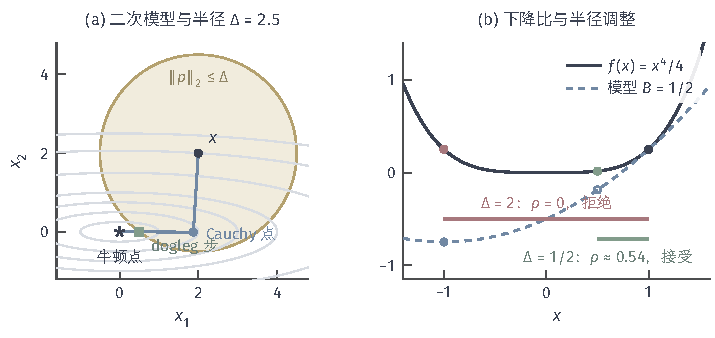
\includegraphics[width=121.1mm]{figures/03-optimization-evolution-and-signals/01-optimization/tikz/c3-trust-region/figure.pdf}
  \caption{信赖域方法。(a) 共同例在$\bm x=(2,2)^\top$处的二次模型等高线与半径$\Delta=2.5$的信赖域（黄色圆盘）。蓝色折线从$\bm x$到Cauchy点，再到位于域外的牛顿点（原点）；绿色方块是折线与边界的交点，即狗腿步。(b) 例~\ref{ex:opt-smooth-trust-region}：$f(x)=x^4/4$与$x=1$处曲率偏小的模型（$B=1/2$）。红色线段是$\Delta=2$的信赖区间，模型最小点$x=-1$处的真实目标（红点）并不低于出发点，$\rho=0$；绿色线段是缩小后的$\Delta=1/2$，候选点$x=1/2$被接受。空心点是模型在候选点的值。}
  \label{fig:opt-smooth-trust-region}
\end{figure*}

\paragraph{收敛条件}
信赖域方法的全局收敛论证需要几项条件同时成立：每轮候选步的预测下降至少是Cauchy点预测下降的固定比例，即$m(\bm0)-m(\bm p)\geq c_1\lVert\bm g\rVert_2\min\{\Delta,\lVert\bm g\rVert_2/\lVert\bm B\rVert_2\}$；模型矩阵一致有界；目标下有界且梯度在相关水平集附近Lipschitz连续；接受规则如算法~\ref{alg:opt-smooth-trust-region}。在这些条件下可以证明$\liminf_{t\to\infty}\lVert\nabla f(\bm x^{(t)})\rVert_2=0$，取$\eta_{\mathrm a}>0$时还有$\lim_{t\to\infty}\lVert\nabla f(\bm x^{(t)})\rVert_2=0$\cite{math-nocedal2006numerical}。论证的骨架是：半径足够小时模型误差相对预测下降可忽略，$\rho$接近$1$，所以半径不会无限缩小；而每次接受都使目标下降一个与梯度相关的量，目标有下界，梯度就不能一直很大。只说“子问题在球内被精确最小化”不能代替这些条件，而模型在球内的全局最小点，也不是原非凸目标的全局最小点。

\subsection{不精确牛顿与Newton--CG}
\label{sec:opt-smooth-newton-cg}

当$d$达到数万乃至更大时，形成并分解$d\times d$的Hessian都不可行。但很多问题可以廉价地计算\term{Hessian向量积}（Hessian-vector product）$\bm v\mapsto\nabla^2f(\bm x)\bm v$：由$\nabla^2f(\bm x)\bm v=\lim_{h\to0}(\nabla f(\bm x+h\bm v)-\nabla f(\bm x))/h$可以用两次梯度差分近似，自动微分则能以常数倍于一次梯度的代价精确计算它。只用这种乘积近似求解牛顿方程的方法，称为\term{不精确牛顿法}（inexact Newton method）；内层用共轭梯度法时称为\term{Newton--CG法}（Newton--CG method）。

\paragraph{内层：截断共轭梯度}
共轭梯度法（CG）在系数矩阵对称正定时求解线性方程，每步一次矩阵向量积，算法与收敛性可参考上文引用的卷一“线性方程与矩阵方程”章。用于$\bm H\bm p=-\bm g$时，$\bm H$可能不定，所以需要在每步检查方向上的曲率；同时规定方程残差$\bm r=\bm H\bm p+\bm g$小到什么程度就停止。

\begin{algorithm}[Newton--CG的内层（线搜索版本）]
\label{alg:opt-smooth-newton-cg}
\begin{algorithmic}[1]
\Require Hessian向量积$\bm v\mapsto\bm H\bm v$，梯度$\bm g\neq\bm0$，精度参数$\vartheta\in(0,1)$
\Ensure 候选方向$\bm p$与停止原因
\State $\bm p_0\gets\bm0$，$\bm r_0\gets\bm g$，$\bm d_0\gets-\bm g$
\For{$j=0,1,2,\dots$}
  \State $\kappa_j\gets\bm d_j^\top\bm H\bm d_j$
  \If{$\kappa_j\leq0$} \State \Return $\bm p_j$（$j=0$时返回$-\bm g$），原因：非正曲率 \EndIf
  \State $a_j\gets\lVert\bm r_j\rVert_2^2/\kappa_j$，$\bm p_{j+1}\gets\bm p_j+a_j\bm d_j$，$\bm r_{j+1}\gets\bm r_j+a_j\bm H\bm d_j$
  \If{$\lVert\bm r_{j+1}\rVert_2\leq\vartheta\lVert\bm g\rVert_2$} \State \Return $\bm p_{j+1}$，原因：残差达标 \EndIf
  \State $b_j\gets\lVert\bm r_{j+1}\rVert_2^2/\lVert\bm r_j\rVert_2^2$，$\bm d_{j+1}\gets-\bm r_{j+1}+b_j\bm d_j$
\EndFor
\end{algorithmic}
\end{algorithm}

算法只在曲率为正时才用它的倒数计算步长，所以每个已接受的内步都使模型下降，返回的$\bm p$是下降方向。外层仍对$\bm p$作Armijo回溯，用原目标决定接受。信赖域版本（Steihaug的截断CG）作两处改动：遇到非正曲率时沿$\bm d_j$走到信赖域边界，新位移越出边界时截在边界上，再交给算法~\ref{alg:opt-smooth-trust-region}按下降比判断。于是内层有三种停止原因：残差达标、遇到非正曲率、触及信赖域边界。实现中应分别记录，因为它们说明不同的情况：第一种说明方程解得够准，后两种说明模型在当前范围内不适合求其驻点。

\paragraph{精度控制与局部收敛阶}
内层解得多准，决定外层能保持多快的局部速度。用随外层变化的参数$\vartheta^{(t)}$规定$\lVert\bm r^{(t)}\rVert_2\leq\vartheta^{(t)}\lVert\bm g^{(t)}\rVert_2$，序列$(\vartheta^{(t)})$称为\term{强迫序列}（forcing sequence）。在定理~\ref{thm:opt-smooth-newton-local}的邻域内（$\nabla^2f\succeq\mu\bm I$，Hessian为$M$-Lipschitz），设$\vartheta^{(t)}\leq\bar\vartheta<1$且接受单位步。由$\bm p=(\bm H^{(t)})^{-1}(-\bm g^{(t)}+\bm r^{(t)})$得$\lVert\bm p\rVert_2\leq(1+\bar\vartheta)\lVert\bm g^{(t)}\rVert_2/\mu\leq2\lVert\bm g^{(t)}\rVert_2/\mu$。新梯度为
\[
  \begin{aligned}
  \bm g^{(t+1)}&=\bm g^{(t)}+\bm H^{(t)}\bm p+\int_0^1\bigl(\nabla^2f(\bm x^{(t)}+s\bm p)-\bm H^{(t)}\bigr)\bm p\,\mathrm ds\\
  &=\bm r^{(t)}+\int_0^1\bigl(\nabla^2f(\bm x^{(t)}+s\bm p)-\bm H^{(t)}\bigr)\bm p\,\mathrm ds ,
  \end{aligned}
\]
取范数得
\begin{equation}
\label{eq:opt-smooth-inexact-newton}
  \lVert\bm g^{(t+1)}\rVert_2\leq\vartheta^{(t)}\lVert\bm g^{(t)}\rVert_2+\frac M2\lVert\bm p\rVert_2^2\leq\Bigl(\vartheta^{(t)}+\frac{2M}{\mu^2}\lVert\bm g^{(t)}\rVert_2\Bigr)\lVert\bm g^{(t)}\rVert_2 .
\end{equation}
括号中的因子说明了三种情形。$\vartheta^{(t)}\leq\bar\vartheta<1$固定时，梯度足够小后因子小于某个$q<1$，梯度范数线性收敛；$\vartheta^{(t)}\to0$时因子趋于零，即\term{超线性收敛}（superlinear convergence）；$\vartheta^{(t)}\leq C\lVert\bm g^{(t)}\rVert_2$时右边是$\lVert\bm g^{(t)}\rVert_2^2$的倍数，恢复二次收敛。这里保证的是梯度范数的收敛阶；在该邻域内$\mu\lVert\bm x-\bm x^\star\rVert_2\leq\lVert\nabla f(\bm x)\rVert_2$，参数误差随之受控。固定内层CG步数并不对应某个确定的$\vartheta$，因为同样步数达到的残差还取决于谱分布与预条件。

\paragraph{内层工作与外层收益}
$\vartheta^{(t)}$越小，内层CG步越多，每步一次Hessian向量积。远离解时二次模型本身就不准确，把模型方程解到很高精度只增加成本，不能改善原目标的下降，所以常见的选择是让$\vartheta^{(t)}$随$\lVert\bm g^{(t)}\rVert_2$一起减小，例如$\vartheta^{(t)}=\min\{1/2,\sqrt{\lVert\bm g^{(t)}\rVert_2}\}$，它在远处宽松、在近处给出超线性收敛。每轮存储只需几个$d$维向量，这是Newton--CG相对于完整牛顿法的主要优势。

\paragraph{CG看不到的方向}
CG只在Krylov子空间$\operatorname{span}\{\bm g,\bm H\bm g,\bm H^2\bm g,\dots\}$中工作，它没有遇到负曲率，不说明$\bm H$半正定。取$\bm H=\operatorname{diag}(1,-1)$，$\bm g=(1,0)^\top$：$\bm H\bm g=\bm g$，Krylov子空间就是$x_1$轴，CG第一步得到$\kappa_0=1>0$、$\bm p_1=(-1,0)^\top$，残差为零，正常结束，完全看不到$x_2$方向的曲率$-1$。所以Newton--CG的“残差达标”不能当作二阶最优性的证据；需要认证没有负曲率时，必须用第~\ref{sec:opt-smooth-nonconvex}节的曲率检测。

\subsection{拟牛顿方法}
\label{sec:opt-smooth-quasi-newton}

Hessian向量积仍要求能对梯度再求导。若只有梯度可用，能否从迭代过程中已经算出的梯度里“拼出”曲率？

\paragraph{割线条件}
走完一步后，我们知道位移和梯度的变化：
\[
  \bm s^{(t)}=\bm x^{(t+1)}-\bm x^{(t)},\qquad\bm y^{(t)}=\nabla f(\bm x^{(t+1)})-\nabla f(\bm x^{(t)}),
\]
由沿线段积分，$\bm y^{(t)}$又可写成
\[
  \bm y^{(t)}=\Bigl(\int_0^1\nabla^2f(\bm x^{(t)}+\tau\bm s^{(t)})\,\mathrm d\tau\Bigr)\bm s^{(t)} .
\]
$\bm y^{(t)}$记录了沿$\bm s^{(t)}$方向的平均曲率作用；对二次目标恰有$\bm y=\bm H\bm s$。\term{拟牛顿法}（quasi-Newton method）要求新的模型矩阵复现这一观测，即\term{割线条件}（secant condition）
\begin{equation}
\label{eq:opt-smooth-secant}
  \bm B^{(t+1)}\bm s^{(t)}=\bm y^{(t)} .
\end{equation}
一维时它唯一确定$B^{(t+1)}=y/s$，正是导数曲线上两点连线的斜率。图~\ref{fig:opt-smooth-secant}(a)取$f(x)=e^x-2x$，$x^{(t)}=0$、$x^{(t+1)}=1$：割线斜率$e-1\approx1.718$介于两端的真实曲率$1$与$e\approx2.718$之间。$d>1$时，割线条件只给出$d$个方程，对称矩阵却有$d(d+1)/2$个自由度，还需要一条规则决定其余部分。

\paragraph{BFGS更新}
BFGS更新\cite{math-nocedal2006numerical}在满足割线条件的前提下，只用两个秩一修正改动旧矩阵：
\begin{equation}
\label{eq:opt-smooth-bfgs}
  \bm B^{(t+1)}=\bm B^{(t)}+\frac{\bm y\bm y^\top}{\bm y^\top\bm s}-\frac{\bm B^{(t)}\bm s\bm s^\top\bm B^{(t)}}{\bm s^\top\bm B^{(t)}\bm s},
\end{equation}
这里省略了$\bm s,\bm y$的上标。直接验证：$\bm B^{(t+1)}\bm s=\bm B^{(t)}\bm s+\bm y-\bm B^{(t)}\bm s=\bm y$。对与$\bm s$正交（在$\bm B^{(t)}$内积下）的方向，第三项不起作用，第二项的作用也只沿$\bm y$，所以更新在“已经观测过的方向”上记住新曲率，其余方向基本保留旧的估计。

\begin{example}[一次BFGS更新保留了什么]
\label{ex:opt-smooth-bfgs}
在共同例上取$\bm B^{(0)}=\bm I$。若位移$\bm s=(0,1)^\top$，则$\bm y=\bm H\bm s=(0,16)^\top$，更新给出$\bm B^{(1)}=\bm I+\operatorname{diag}(0,16)-\operatorname{diag}(0,1)=\operatorname{diag}(1,16)$，一步就得到真实Hessian，因为$\bm s$恰是特征方向。若位移$\bm s=(1,1)^\top$，则$\bm y=(1,16)^\top$，$\bm y^\top\bm s=17$，$\bm s^\top\bm B^{(0)}\bm s=2$，
\[
  \bm B^{(1)}=\bm I+\frac1{17}\begin{pmatrix}1&16\\16&256\end{pmatrix}-\frac12\begin{pmatrix}1&1\\1&1\end{pmatrix}=\frac1{34}\begin{pmatrix}19&15\\15&529\end{pmatrix}.
\]
可以核对$\bm B^{(1)}\bm s=(1,16)^\top=\bm y$。沿$\bm s$它与$\bm H$完全一致，沿与之正交的$(1,-1)^\top$，二次型$\bm v^\top\bm B^{(1)}\bm v=518/34\approx15.2$，而真实值是$17$，只是部分地学到了。图~\ref{fig:opt-smooth-secant}(b)把三个矩阵画成椭圆$\bm v^\top\bm M\bm v=1$：$\bm B^{(1)}$的椭圆与$\bm H$的椭圆恰好在$\pm\bm s/\sqrt{17}$处相交。
\end{example}

\begin{figure}[htbp]
  \centering
  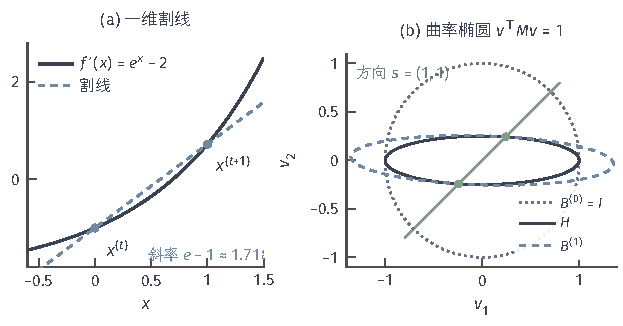
\includegraphics[width=105.5mm]{figures/03-optimization-evolution-and-signals/01-optimization/tikz/c3-secant/figure.pdf}
  \caption{割线条件怎样拼出曲率。(a) $f'(x)=e^x-2$在$x^{(t)}=0$与$x^{(t+1)}=1$两点的割线（蓝色虚线），斜率$e-1$是这段区间上的平均曲率。(b) 例~\ref{ex:opt-smooth-bfgs}中三个矩阵$\bm M$的曲率椭圆$\bm v^\top\bm M\bm v=1$：灰色点线为初始$\bm B^{(0)}=\bm I$，黑色为真实$\bm H=\operatorname{diag}(1,16)$，蓝色虚线为沿$\bm s=(1,1)^\top$更新一次后的$\bm B^{(1)}$。绿色直线是$\bm s$方向，$\bm B^{(1)}$与$\bm H$的椭圆在绿点处重合。}
  \label{fig:opt-smooth-secant}
\end{figure}

\paragraph{曲率条件与线搜索}
BFGS更新保持正定的关键是\term{曲率条件}（curvature condition）$\bm y^\top\bm s>0$。设$\bm B^{(t)}\succ\bm0$且$\bm y^\top\bm s>0$，对任意$\bm v\neq\bm0$，由$\bm B^{(t)}$内积的Cauchy--Schwarz不等式，$\bm v^\top\bm B^{(t)}\bm v-(\bm s^\top\bm B^{(t)}\bm v)^2/(\bm s^\top\bm B^{(t)}\bm s)\geq0$，等号仅在$\bm v$与$\bm s$平行时成立，而此时$(\bm y^\top\bm v)^2/(\bm y^\top\bm s)>0$；两部分相加即$\bm v^\top\bm B^{(t+1)}\bm v>0$。强凸目标总满足曲率条件；一般目标上，线搜索要额外保证它。只缩短步长的Armijo回溯做不到这一点，需要再加上\term{Wolfe曲率条件}（Wolfe curvature condition）
\[
  \nabla f(\bm x+\eta\bm p)^\top\bm p\geq c_2\,\nabla f(\bm x)^\top\bm p,\qquad 0<c<c_2<1,
\]
它排除了步长过短、斜率还很陡的点。满足它时$\bm y^\top\bm s=\eta\bigl(\nabla f(\bm x+\eta\bm p)-\nabla f(\bm x)\bigr)^\top\bm p\geq\eta(c_2-1)\nabla f(\bm x)^\top\bm p>0$。若某一步观测到的曲率不可靠，实现中可以跳过该次更新或对$\bm y$作阻尼修正。

\paragraph{逆近似与L-BFGS}
实际计算中维护逆近似$\bm C=\bm B^{-1}$更方便，方向为$-\bm C\bm g$，由Sherman--Morrison--Woodbury公式，式~\eqref{eq:opt-smooth-bfgs}等价于
\[
  \bm C^{(t+1)}=\bigl(\bm I-\omega\bm s\bm y^\top\bigr)\bm C^{(t)}\bigl(\bm I-\omega\bm y\bm s^\top\bigr)+\omega\bm s\bm s^\top,\qquad\omega=\frac1{\bm y^\top\bm s}.
\]
每轮$O(d^2)$运算和$O(d^2)$存储，不需要解线性方程。$d$很大时连$d^2$也存不下。\term{有限内存拟牛顿法}（limited-memory BFGS，L-BFGS）只保存最近$r$对$(\bm s_i,\bm y_i)$，从一个简单的初始逆近似$\bm C_0$（常取$\gamma\bm I$，$\gamma=\bm s^\top\bm y/\bm y^\top\bm y$取自最近一对）出发，隐式地施加这$r$次更新，用两次循环直接算出方向$\bm C\bm g$，而不形成矩阵。

\begin{algorithm}[L-BFGS的双循环递推]
\label{alg:opt-smooth-lbfgs}
\begin{algorithmic}[1]
\Require 梯度$\bm g$，最近$r$对$(\bm s_i,\bm y_i)$（$i=k-r,\dots,k-1$，均满足$\bm y_i^\top\bm s_i>0$），初始尺度$\gamma>0$
\Ensure $\bm z=\bm C\bm g$，方向取$-\bm z$
\State $\bm q\gets\bm g$
\For{$i=k-1,k-2,\dots,k-r$} \Comment{从新到旧}
  \State $\omega_i\gets1/(\bm y_i^\top\bm s_i)$，$\alpha_i\gets\omega_i\bm s_i^\top\bm q$，$\bm q\gets\bm q-\alpha_i\bm y_i$
\EndFor
\State $\bm z\gets\gamma\bm q$
\For{$i=k-r,\dots,k-1$} \Comment{从旧到新}
  \State $b\gets\omega_i\bm y_i^\top\bm z$，$\bm z\gets\bm z+(\alpha_i-b)\bm s_i$
\EndFor
\end{algorithmic}
\end{algorithm}

每轮约$4rd$次乘加，存储$2rd$个数；$r$常取$5$到$20$。完整BFGS在$\bm x^\star$处Hessian正定、Hessian在邻域内Lipschitz、单位步优先尝试且合格即接受等条件下，局部超线性收敛；其证明依赖$\bm B^{(t)}$沿实际位移方向逐渐逼近真实Hessian\cite{math-nocedal2006numerical}。L-BFGS不断丢弃旧信息，这一逼近一般不成立，完整BFGS的超线性结论不能直接移用；它的实际效果通常很好，但理论保证要按有限记忆的形式另行说明。另一个常被提到的性质，“正定二次目标上用精确线搜索的BFGS至多$d$步终止”，也只在精确线搜索这一特殊条件下成立。

\subsection{立方正则化（补充）}
\label{sec:opt-smooth-cubic}

信赖域用硬半径限制位移；本小节介绍一种用光滑的惩罚限制位移的模型，它把Hessian的Lipschitz常数直接写进模型，因而在非凸目标上也能给出清楚的下降量与复杂度。初读可以跳过，第~\ref{sec:opt-smooth-nonconvex}节只用到其中的结论。

\paragraph{三阶余项与立方模型}
若Hessian在包含线段$[\bm x,\bm x+\bm p]$的凸区域上$M$-Lipschitz，与下降引理同样沿线段积分两次，得
\[
  f(\bm x+\bm p)\leq f(\bm x)+\langle\bm g,\bm p\rangle+\frac12\bm p^\top\bm H\bm p+\frac M6\lVert\bm p\rVert_2^3 .
\]
\term{立方正则化}（cubic regularization）的牛顿法\cite{nesterov2006cubic}在第$t$轮最小化
\begin{equation}
\label{eq:opt-smooth-cubic-model}
  m_\sigma(\bm p)=f(\bm x)+\langle\bm g,\bm p\rangle+\frac12\bm p^\top\bm H\bm p+\frac\sigma3\lVert\bm p\rVert_2^3,\qquad\sigma>0 .
\end{equation}
取$\sigma\geq M/2$时，$m_\sigma$是$f(\bm x+\bm p)$的上界，模型下降就保证实际下降，这是下降引理在二阶上的对应物。立方项在远处的增长快过二次项，即使$\bm H$不定，模型也有全局最小点；它惩罚的是本轮位移，不改变原目标。图~\ref{fig:opt-smooth-cubic-model}取$f(x)=x^4/4-x^2/2$，在$x=0.2$处$g=-0.192$、$H=-0.88$，二次模型开口向下、没有最小点；区间$[-1,1]$上$|f'''|\leq6$，取$\sigma=3$，立方模型的最小点为$s\approx0.439$，到达$x+s\approx0.639$，目标从$-0.0196$降到约$-0.163$。

\begin{figure}[htbp]
  \centering
  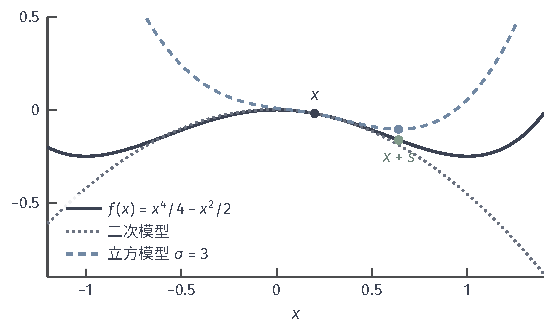
\includegraphics[width=92.9mm]{figures/03-optimization-evolution-and-signals/01-optimization/tikz/c3-cubic-model/figure.pdf}
  \caption{$f(x)=x^4/4-x^2/2$（黑）在$x=0.2$处的局部模型。二次模型（灰色点线）的曲率$-0.88$为负，向两侧无界下降；加上$\tfrac\sigma3|p|^3$（$\sigma=3$）后的立方模型（蓝色虚线）在区间$[-1,1]$上位于$f$之上，最小点给出$s\approx0.439$。蓝点是模型值约$-0.104$，绿点是真实目标约$-0.163$。}
  \label{fig:opt-smooth-cubic-model}
\end{figure}

\paragraph{模型最小点的刻画}
可以证明，$\bm s$是$m_\sigma$的全局最小点，当且仅当下面两式同时成立\cite{nesterov2006cubic}：
\[
  \bm g+\bm H\bm s+\sigma\lVert\bm s\rVert_2\bm s=\bm0,\qquad\bm H+\sigma\lVert\bm s\rVert_2\bm I\succeq\bm0 .
\]
第一式是模型的驻点方程，第二式是附加的曲率条件；只满足第一式的点可能是模型的鞍点或局部最大点，所以近似求解时只看模型梯度小不够。图中$H+\sigma s=-0.88+3\times0.439\approx0.44\geq0$，两式都成立。

\paragraph{下降量与新点的梯度}
设$\sigma\geq M/2$，$\bm s$满足上面两式。由驻点方程，$\langle\bm g,\bm s\rangle=-\bm s^\top\bm H\bm s-\sigma\lVert\bm s\rVert_2^3$，代入模型得
\[
  \begin{aligned}
  m_\sigma(\bm s)-f(\bm x)&=-\frac12\bm s^\top\bm H\bm s-\frac{2\sigma}3\lVert\bm s\rVert_2^3\\
  &\leq\frac\sigma2\lVert\bm s\rVert_2^3-\frac{2\sigma}3\lVert\bm s\rVert_2^3=-\frac\sigma6\lVert\bm s\rVert_2^3,
  \end{aligned}
\]
其中用了曲率条件给出的$\bm s^\top\bm H\bm s\geq-\sigma\lVert\bm s\rVert_2^3$。所以$f(\bm x)-f(\bm x+\bm s)\geq\tfrac\sigma6\lVert\bm s\rVert_2^3$。另一方面，新点的梯度
\[
  \begin{aligned}
  \nabla f(\bm x+\bm s)&=\bm g+\bm H\bm s+\int_0^1\bigl(\nabla^2f(\bm x+\tau\bm s)-\bm H\bigr)\bm s\,\mathrm d\tau\\
  &=-\sigma\lVert\bm s\rVert_2\bm s+\int_0^1\bigl(\nabla^2f(\bm x+\tau\bm s)-\bm H\bigr)\bm s\,\mathrm d\tau,
  \end{aligned}
\]
故$\lVert\nabla f(\bm x+\bm s)\rVert_2\leq(\sigma+M/2)\lVert\bm s\rVert_2^2$。把两式连起来：只要新点的梯度范数大于$\varepsilon$，本步的下降就至少为$\tfrac\sigma6\bigl(\varepsilon/(\sigma+M/2)\bigr)^{3/2}$。若$f$下有界，这样的步至多有$O(\varepsilon^{-3/2})$个，于是在$O(\varepsilon^{-3/2})$轮内得到$\lVert\nabla f\rVert_2\leq\varepsilon$的点；梯度下降的对应界是$O(\varepsilon^{-2})$（定理~\ref{thm:opt-smooth-gd-nonconvex}）。

\paragraph{这个复杂度计了什么}
$O(\varepsilon^{-3/2})$数的是外层轮数，也就是目标、梯度与Hessian的求值次数。每轮的子问题本身需要求解，精确求解通常要特征分解或解一个一维非线性方程，代价可达$O(d^3)$。用近似子问题解代替时，近似解必须同时达到上面用到的模型下降、驻点方程残差和曲率条件的相应精度，复杂度结论才能保留。$M$未知时，实现中按与下降比~\eqref{eq:opt-smooth-trust-ratio}同样的方式根据接受结果调整$\sigma$。

\section{非凸目标与鞍点}
\label{sec:opt-smooth-nonconvex}

前两节的保证在非凸目标上只剩下“梯度变小”。本节研究这句话究竟说了什么：下降方法可能停在哪些点，梯度小与到达局部最小点相差多远；以及在已有梯度和曲率信息的前提下，怎样主动离开那些不是最小点的驻点。全节分析离散迭代，连续时间的梯度流不能代替离散算法的结论。

\subsection{驻点残差与负曲率下降}
\label{sec:opt-smooth-negative-curvature}

\paragraph{梯度趋零说明了什么}
第~\ref{chap:optimization}章给出了内点处的最优条件：局部最小点必须满足$\nabla f=\bm0$与$\nabla^2f\succeq\bm0$；驻点处$\nabla^2f\succ\bm0$则足以保证严格局部最小。定理~\ref{thm:opt-smooth-gd-nonconvex}保证的是$\nabla f(\bm x^{(t)})\to\bm0$，这与“迭代收敛到驻点”之间还隔着两步。第一，梯度趋零不意味着迭代有界：$f(x)=e^{-x}$在$[0,\infty)$上下有界且$L=1$光滑，从$x^{(0)}=0$用$\eta=1$出发，迭代单调右移、梯度趋于零，却根本没有驻点可以趋近。第二，若迭代有界，由梯度的连续性，每个聚点都是驻点；但聚点可能不止一个，仅凭梯度趋零推不出整个序列收敛到某一点。所以“返回梯度小的点”这句话，只对应“近似一阶驻点”。

\paragraph{驻点的种类}
驻点处若$\nabla^2f$有负特征值，就称为\term{严格鞍点}（strict saddle point）。这个名称约定也覆盖局部最大点，因为它们同样有负曲率方向；关键在于负曲率提供了离开的方向。为了区分“梯度小”的点里哪些可能接近局部最小点，引入双容差：若
\[
  \lVert\nabla f(\bm x)\rVert_2\leq\varepsilon_g,\qquad\lambda_{\min}\bigl(\nabla^2f(\bm x)\bigr)\geq-\varepsilon_H,
\]
就称$\bm x$为\term{近似二阶驻点}（approximate second-order stationary point）。它排除了曲率明显为负的鞍点，但仍不是局部最小性的充分条件。$f(x_1,x_2)=x_1^4-x_2^4$在原点处梯度和Hessian都为零，满足任意容差下的近似二阶条件，却是鞍点：沿$x_1$轴目标为正、沿$x_2$轴为负。高阶平坦的鞍点用一阶和二阶信息都看不出来。

\paragraph{沿负曲率方向下降}
在鞍点附近，梯度很小，梯度步几乎不动；但若已经知道一个负曲率方向，就能用二阶信息得到可量化的下降。设单位向量$\bm v$满足$\bm v^\top\nabla^2f(\bm x)\bm v\leq-\gamma<0$，称为\term{负曲率方向}（negative curvature direction）。必要时把$\bm v$换成$-\bm v$，使$\langle\nabla f(\bm x),\bm v\rangle\leq0$。若Hessian在包含$[\bm x,\bm x+\alpha\bm v]$的凸区域上$M$-Lipschitz，由立方正则化小节的三阶余项界，
\[
  f(\bm x+\alpha\bm v)\leq f(\bm x)+\alpha\langle\nabla f(\bm x),\bm v\rangle+\frac{\alpha^2}2\bm v^\top\nabla^2f(\bm x)\bm v+\frac M6\alpha^3
  \leq f(\bm x)-\frac\gamma2\alpha^2+\frac M6\alpha^3 .
\]
右边在$\alpha=2\gamma/M$处最小，给出
\begin{equation}
\label{eq:opt-smooth-negative-curvature-decrease}
  f\Bigl(\bm x+\frac{2\gamma}M\bm v\Bigr)\leq f(\bm x)-\frac{2\gamma^3}{3M^2}.
\end{equation}
下降量只取决于负曲率的大小和Hessian的变化速度，与梯度多小无关，正好补上梯度步在鞍点附近的不足。例如$f(\bm x)=\tfrac14x_1^4-\tfrac12x_1^2+\tfrac12x_2^2$在原点有$\nabla^2f=\operatorname{diag}(-1,1)$，取$\bm v=(1,0)^\top$、$\gamma=1$；在$|x_1|\leq1$上$\partial^3f/\partial x_1^3=6x_1$，$M=6$。步长$\alpha=1/3$给出$f(1/3,0)\approx-0.0525$，不高于界$-2/(3\cdot36)\approx-0.0185$。

\paragraph{检测负曲率的代价}
式~\eqref{eq:opt-smooth-negative-curvature-decrease}的前提是手里真有一个负曲率方向。寻找它要计算Hessian的最小特征值或其近似，例如用Lanczos方法，每步一次Hessian向量积；检测本身有误差，所得的$\gamma$只是Rayleigh商的估计，应先核实$\bm v^\top\nabla^2f(\bm x)\bm v$，再用原目标检验位移。这些计算都应计入算法的成本。用正定近似代替真实Hessian是检测不到负曲率的：BFGS矩阵、修正牛顿的$\bm H+\bm E$按构造总是正定的，它们没有负特征值不说明真实Hessian没有；上一节也说明，Newton--CG的内层只看Krylov子空间，同样可能漏掉负曲率。

\subsection{扰动与逃离鞍点}
\label{sec:opt-smooth-perturbed}

不计算Hessian，只用梯度，能否离开鞍点？先看梯度下降在鞍点附近怎样运动。对上一小节的例子，梯度下降的两个坐标各自演化：
\[
  x_1^{(t+1)}=x_1^{(t)}+\eta\bigl(x_1^{(t)}-(x_1^{(t)})^3\bigr),\qquad x_2^{(t+1)}=(1-\eta)x_2^{(t)} .
\]
在原点附近$x_1$每步约乘以$1+\eta$，$x_2$每步乘以$1-\eta$。从$x_1^{(0)}=0$出发，$x_1$永远为零，迭代沿$x_2$轴收敛到鞍点；这条轴就是鞍点的稳定流形。只要$x_1^{(0)}\neq0$，哪怕非常小，$x_1$就会按几何级数放大，迭代最终离开鞍点、落入某个最小点$(\pm1,0)$的吸引域。图~\ref{fig:opt-smooth-saddle-escape}取$\eta=0.2$：从$(10^{-3},1.5)^\top$出发的路径先沿$x_2$轴下滑，在鞍点附近停留十余步，到第$35$步$x_1$才超过$0.5$，随后落到最小点$(1,0)$；它在徘徊处梯度很小，若此时按梯度容差停止，就会把鞍点附近的点当作结果返回。

\begin{figure*}[htbp]
  \centering
  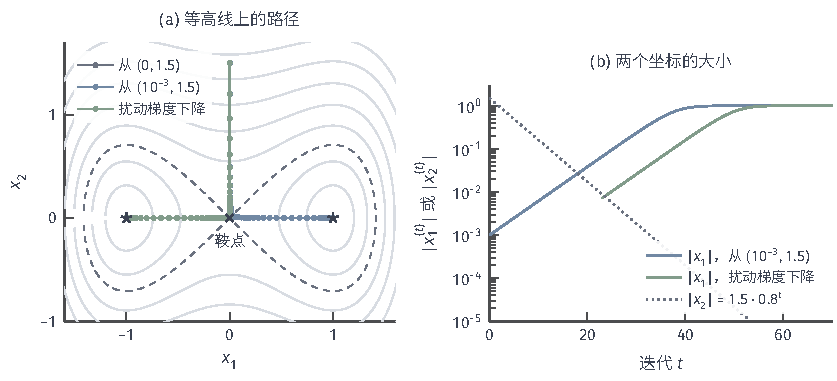
\includegraphics[width=141.7mm]{figures/03-optimization-evolution-and-signals/01-optimization/tikz/c3-saddle-escape/figure.pdf}
  \caption{目标$f(\bm x)=\tfrac14x_1^4-\tfrac12x_1^2+\tfrac12x_2^2$上步长$\eta=0.2$的梯度下降，叉号为原点处的严格鞍点，星号为最小点$(\pm1,0)$，灰色虚线是零等值线。(a) 从$(0,1.5)^\top$出发（灰）沿稳定流形收敛到鞍点；从$(10^{-3},1.5)^\top$出发（蓝）先接近鞍点再离开；扰动梯度下降（绿）从$(0,1.5)^\top$出发，在梯度降到$10^{-2}$时（第23步）加入半径$10^{-2}$内的均匀扰动，随后离开。(b) 对数坐标下$|x_1^{(t)}|$与$|x_2^{(t)}|$：负曲率坐标每步约放大$1.2$倍（直线上升），正曲率坐标每步乘以$0.8$。}
  \label{fig:opt-smooth-saddle-escape}
\end{figure*}

\paragraph{普通梯度下降的渐近避鞍}
上面的例子说明，收敛到严格鞍点需要初值恰好落在一个“零测”的稳定流形上。这一观察有严格的版本：设$f$二阶连续可微、梯度全局$L$-Lipschitz，步长$0<\eta<1/L$，初值服从对Lebesgue测度绝对连续的分布，则对每个严格鞍点，梯度下降收敛到它的概率为零\cite{lee2016gradient}。这里的随机性只来自初值，之后的迭代完全确定。结论有三个限度。它是渐近的，不说明离开需要多少步，图中蓝色路径若初值更接近稳定流形，徘徊时间会按$\log(1/|x_1^{(0)}|)$增长。它只排除收敛到严格鞍点，要说“几乎必然收敛到局部最小点”，还需迭代本身收敛、所有非最小驻点都是严格鞍点等额外条件。它针对固定步长的梯度下降，不能直接搬到回溯步长、动量或随机梯度。

\paragraph{扰动梯度下降}
要得到有限步的保证，可以在可疑区域主动加一点随机扰动，把迭代推离稳定流形。\term{扰动梯度下降}（perturbed gradient descent）的骨架如下\cite{jin2017escape}。

\begin{algorithm}[扰动梯度下降的骨架]
\label{alg:opt-smooth-pgd}
\begin{algorithmic}[1]
\Require 初值$\bm x^{(0)}$，步长$\eta$，梯度阈值$g_{\mathrm{th}}$，扰动半径$r$，观察窗口长度$t_{\mathrm{th}}$，下降阈值$f_{\mathrm{th}}$
\Ensure 返回点
\State $t_{\mathrm{p}}\gets-\infty$（上次扰动的时刻）
\For{$t=0,1,2,\dots$}
  \If{$\lVert\nabla f(\bm x^{(t)})\rVert_2\leq g_{\mathrm{th}}$ 且 $t-t_{\mathrm p}>t_{\mathrm{th}}$}
    \State 保存基点$\tilde{\bm x}\gets\bm x^{(t)}$及$f(\tilde{\bm x})$，$t_{\mathrm p}\gets t$
    \State $\bm x^{(t)}\gets\tilde{\bm x}+\bm\xi$，$\bm\xi$在半径$r$的球内均匀抽取
  \EndIf
  \If{$t-t_{\mathrm p}=t_{\mathrm{th}}$ 且 $f(\bm x^{(t)})>f(\tilde{\bm x})-f_{\mathrm{th}}$}
    \State \Return $\tilde{\bm x}$ \Comment{窗口内没有足够下降，基点视为近似二阶驻点}
  \EndIf
  \State $\bm x^{(t+1)}\gets\bm x^{(t)}-\eta\nabla f(\bm x^{(t)})$
\EndFor
\end{algorithmic}
\end{algorithm}

算法的逻辑是一个检验：梯度小时，在基点周围随机挪一点，再跑一段普通梯度下降；若基点附近有明显的负曲率，扰动几乎必然带有该方向的分量，这个分量在窗口内被放大，目标下降至少$f_{\mathrm{th}}$；若窗口结束时没有这么多下降，就推断基点附近没有明显的负曲率，返回基点。扰动不是“随便加噪声”：它只在规定条件下触发，半径、窗口长度和阈值都由$L$、$M$、目标精度$\varepsilon$、失败概率$\delta$与初始目标差联合确定，返回的是保存的基点而不是扰动后的点。图~\ref{fig:opt-smooth-saddle-escape}中的绿色路径从稳定流形上出发，普通梯度下降会停在鞍点；第$23$步的扰动把$x_1$从$0$推到约$-0.007$，之后与蓝色路径一样离开，只是落向另一个最小点$(-1,0)$。

\paragraph{有限步保证与它的含义}
在$f$二阶连续可微、梯度$L$-Lipschitz、Hessian $M$-Lipschitz、$f$下有界等条件下，适当选取参数的扰动梯度下降以至少$1-\delta$的概率返回满足
\[
  \lVert\nabla f(\bm x)\rVert_2\leq\varepsilon,\qquad\lambda_{\min}\bigl(\nabla^2f(\bm x)\bigr)\geq-\sqrt{M\varepsilon}
\]
的点，所需梯度计算次数为$\tilde O\bigl(L(f(\bm x^{(0)})-f_{\inf})/\varepsilon^2\bigr)$，其中$\tilde O$隐去了关于$d$、$1/\delta$等的对数因子\cite{jin2017escape}。与定理~\ref{thm:opt-smooth-gd-nonconvex}相比，梯度计算次数只多了对数因子，却额外控制了负曲率。与上一小节的普通梯度下降结论对照：前者是对初值随机性的渐近陈述，后者是对算法内部随机扰动的有限步、高概率陈述，两者的条件和结论都不同。最后要记住，近似二阶驻点仍不等于局部最小点（高阶平坦的鞍点可以满足它），更不等于全局最小点：目标若有不好的局部最小点，任何局部方法都可能停在那里，要排除这种情况，需要对目标的整体形状另作分析。

\section{算法精度与计算成本}
\label{sec:opt-smooth-accuracy-cost}

前面各节为每个算法给出了各自的保证，但这些保证衡量的对象不同：有的控制目标差，有的控制梯度，有的控制到最小点的距离；有的数迭代轮数，有的只描述进入邻域之后的行为。本节固定同一个优化问题，研究两件事：在同一误差标准下，各方法返回的候选有多准确、为此付出多少工作；以及实际计算中的误差怎样改变这个候选。问题本身的数据变化时最优解怎样移动，是另一类问题，留给下一节。第~\ref{chap:optimization}章已经区分了目标误差、解误差与可计算的残差，并把总成本写成每轮代价与轮数的乘积；本节把这些语言用到光滑优化的具体方法上。

\subsection{收敛速度与总计算成本}
\label{sec:opt-smooth-rates-cost}

\paragraph{三种误差之间的换算}
目标差$f(\bm x)-f^\star$、梯度残差$\lVert\nabla f(\bm x)\rVert_2$和参数误差$\lVert\bm x-\bm x^\star\rVert_2$之间的换算，每个方向都需要自己的条件。

第一，$L$光滑且$f^\star=\inf f>-\infty$时，目标差控制梯度：
\begin{equation}
\label{eq:opt-smooth-gap-controls-gradient}
  \frac1{2L}\lVert\nabla f(\bm x)\rVert_2^2\leq f(\bm x)-f^\star .
\end{equation}
证明只需在式~\eqref{eq:opt-smooth-gd-one-step}中取$\eta=1/L$：$f^\star\leq f(\bm x-\nabla f(\bm x)/L)\leq f(\bm x)-\lVert\nabla f(\bm x)\rVert_2^2/(2L)$。这个方向不需要凸性。

第二，反方向需要曲率的下界。若$f$可微且$\mu$强凸，第~\ref{chap:optimization}章的一阶下界$f(\bm y)\geq f(\bm x)+\langle\nabla f(\bm x),\bm y-\bm x\rangle+\tfrac\mu2\lVert\bm y-\bm x\rVert_2^2$对$\bm y$取最小，右边的最小值是$f(\bm x)-\lVert\nabla f(\bm x)\rVert_2^2/(2\mu)$，于是
\[
  f(\bm x)-f^\star\leq\frac1{2\mu}\lVert\nabla f(\bm x)\rVert_2^2,\qquad\frac\mu2\lVert\bm x-\bm x^\star\rVert_2^2\leq f(\bm x)-f^\star,
\]
后一式是第~\ref{chap:optimization}章强凸误差控制的结论。没有曲率下界时，小梯度不说明小目标差：$f(x)=\tfrac\epsilon2x^2$的梯度是$\epsilon x$，目标差是$\tfrac\epsilon2x^2=g^2/(2\epsilon)$，$\epsilon$很小时梯度为$10^{-3}$的点，目标差可以任意大。

\paragraph{PL条件}
强凸性同时保证了唯一最小点和梯度对目标差的控制。线性收敛其实只需要后一半。设$f$可微且$f^\star=\inf f>-\infty$，若存在$\mu>0$使
\begin{equation}
\label{eq:opt-smooth-pl}
  \frac12\lVert\nabla f(\bm x)\rVert_2^2\geq\mu\bigl(f(\bm x)-f^\star\bigr)\qquad\text{对所有}\ \bm x ,
\end{equation}
就说$f$满足\term{Polyak--Łojasiewicz条件}（PL condition），简称PL条件\cite{karimi2016pl}。它用梯度范数的平方控制目标差。把它与步长$1/L$的单步下降式~\eqref{eq:opt-smooth-gd-one-step}组合：
\[
  f(\bm x^+)-f^\star\leq f(\bm x)-f^\star-\frac1{2L}\lVert\nabla f(\bm x)\rVert_2^2\leq\Bigl(1-\frac\mu L\Bigr)\bigl(f(\bm x)-f^\star\bigr),
\]
所以$L$光滑且满足PL条件时，梯度下降的目标差按$(1-\mu/L)^t$线性收敛。由式~\eqref{eq:opt-smooth-gap-controls-gradient}，PL常数必然满足$\mu\leq L$，收缩因子落在$[0,1)$中。$\mu$强凸的可微函数满足PL条件，反过来不成立。$f(\bm x)=\tfrac12(x_1-x_2)^2$凸但不强凸，最小点构成整条直线$x_1=x_2$，而$\tfrac12\lVert\nabla f\rVert_2^2=(x_1-x_2)^2=2f$，PL条件以$\mu=2$成立；$f(x)=x^2+3\sin^2x$甚至不凸（$f''(\pi/2)=-4$），也满足PL条件\cite{karimi2016pl}。所以PL条件给出目标差的线性速度，却不保证凸性，也不保证唯一的参数解；在多解时，“参数误差”需要改为到解集的距离。

\paragraph{各类保证的汇总}
表~\ref{tab:opt-smooth-rates}按误差对象汇总本章的主要速度结论。同一行内的条件、误差对象与返回点一起构成结论，不能拆开互换；不同行之间也不能排成一个无条件的优劣顺序，例如牛顿法的二次收敛只在局部邻域内成立，而梯度下降的$O(1/T)$是从任意初值出发的全局结论。

\begin{table*}[htbp]
  \centering
  \small
  \begin{tabularx}{\linewidth}{@{}>{\raggedright\arraybackslash}p{0.27\linewidth}>{\raggedright\arraybackslash}X>{\raggedright\arraybackslash}p{0.16\linewidth}>{\raggedright\arraybackslash}p{0.2\linewidth}@{}}
    \toprule
    条件 & 算法与返回点 & 误差对象 & 速度 \\
    \midrule
    $L$光滑，下有界 & 梯度下降（固定步长或回溯），历史最佳点 & 梯度范数 & $\min_{t<T}\lVert\nabla f\rVert_2=O(T^{-1/2})$ \\
    凸，$L$光滑，最小点存在 & 梯度下降，最后一点 & 目标差 & $O(1/T)$ \\
    同上 & Nesterov方法，最后一点 & 目标差 & $O(1/T^2)$ \\
    $L$光滑，PL条件 & 梯度下降$\eta=1/L$，最后一点 & 目标差 & $(1-\mu/L)^T$ \\
    正定二次，谱界已知 & 梯度下降／重球法，最佳参数 & 参数误差 & 因子$\tfrac{\kappa-1}{\kappa+1}$／$\tfrac{\sqrt\kappa-1}{\sqrt\kappa+1}$ \\
    Hessian $M$-Lipschitz，下有界 & 立方正则化，精确模型步 & 新点梯度范数 & $O(\varepsilon^{-3/2})$轮 \\
    非退化最小点的邻域 & 牛顿法／不精确牛顿／完整BFGS & 参数误差或梯度 & 二次／依强迫序列／超线性 \\
    \bottomrule
  \end{tabularx}
  \caption{光滑优化的代表性速度结论。$T$为迭代轮数，$\varepsilon$为梯度容差。最后一行是局部收敛阶，只描述进入邻域之后的行为。}
  \label{tab:opt-smooth-rates}
\end{table*}

\paragraph{每轮代价}
比较方法时，要在同一误差标准下合计全部工作：函数值、梯度、Hessian或Hessian向量积的计算次数，线搜索中被拒绝的试探，线性代数运算，以及存储。对$d$维稠密问题，各方法每轮的主要代价大致如下：梯度下降一次梯度加上线搜索的若干次函数值，存储$O(d)$；重球法与Nesterov方法同样一次梯度，多存一个向量；牛顿法形成Hessian并作Cholesky分解，运算$O(d^3)$、存储$O(d^2)$；Newton--CG若内层做$k$步，代价是$k$次Hessian向量积加$O(kd)$次向量运算，存储$O(d)$；BFGS每轮$O(d^2)$运算与存储；L-BFGS为$O(rd)$。每轮便宜不等于总成本低，轮数少也不等于总成本低，两者必须相乘。

\paragraph{同一问题上的比较}
图~\ref{fig:opt-smooth-convergence-cost}用一个二维非二次目标\cite{math-boyd2004convex}
\[
  f(\bm x)=e^{x_1+3x_2-0.1}+e^{x_1-3x_2-0.1}+e^{-x_1-0.1}
\]
比较三种方法，它的最小点为$(-\tfrac12\ln2,0)^\top$，$f^\star=2\sqrt2e^{-0.1}\approx2.559$。三种方法从$(-1,0.8)^\top$出发，都用$\bar\eta=1$、$\gamma=1/2$、$c=10^{-4}$的回溯，BFGS从$\bm C^{(0)}=\bm I$开始。成本按如下约定计数：每次函数值记$1$，每次梯度记$1$，每次Hessian记$d=2$（相当于用$d$次梯度差分形成它），二维线性代数的运算忽略不计。达到$f-f^\star<10^{-8}$时，梯度下降用了$20$轮、成本$96$；BFGS用了$7$轮、成本$19$；阻尼牛顿法用了$4$轮、成本$18$。按轮数看，牛顿法远远领先；按成本看，它与BFGS相当，因为每轮的Hessian要多付$2$个单位。$d$增大时，牛顿法的Hessian成本按$d$倍、分解按$d^3$增长，BFGS的每轮成本按$d^2$增长，比较结果会随之改变。这个例子只说明比较的方法，不能推广成某种方法普遍更好。

\begin{figure*}[htbp]
  \centering
  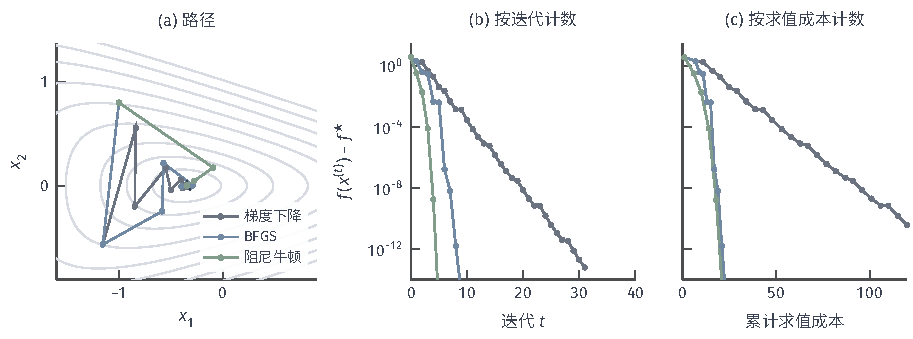
\includegraphics[width=154.6mm]{figures/03-optimization-evolution-and-signals/01-optimization/tikz/c3-convergence-cost/figure.pdf}
  \caption{二维目标$f(\bm x)=e^{x_1+3x_2-0.1}+e^{x_1-3x_2-0.1}+e^{-x_1-0.1}$上三种方法的比较，初值$(-1,0.8)^\top$，均用Armijo回溯（$\bar\eta=1$，$\gamma=1/2$，$c=10^{-4}$）。(a) 等高线上的路径，星号为最小点。(b) 目标差随迭代轮数的变化（对数坐标）：梯度下降（灰）线性下降，BFGS（蓝）后期超线性，阻尼牛顿（绿）最后几步二次收敛。(c) 同一目标差随累计求值成本的变化，函数值与梯度各记$1$，Hessian记$2$；牛顿法与BFGS的差距在这一计数下基本消失。}
  \label{fig:opt-smooth-convergence-cost}
\end{figure*}

在共同例这样的正定二次目标上，比较可以写成公式。梯度下降以最佳固定步长每轮收缩$(\kappa-1)/(\kappa+1)$，把误差缩小到$\varepsilon$倍约需$\tfrac{\kappa}{2}\ln(1/\varepsilon)$轮；重球法约需$\tfrac{\sqrt\kappa}2\ln(1/\varepsilon)$轮，两者每轮都是一次梯度，所以按轮数比较就是按成本比较。$\kappa=10^4$、$\varepsilon=10^{-6}$时，前者约$6.9\times10^4$轮，后者约$690$轮。牛顿法在二次目标上一步到达，但这一步解的线性方程，本身就是原问题。

\subsection{计算误差的传播}
\label{sec:opt-smooth-error-propagation}

到目前为止，每一步都被当作精确执行。实际计算中，梯度可能只是近似值（例如由有限差分或截断的内层迭代得到），求出的位移可能不精确，位移加到参数上时还有舍入。这些误差不会让上一小节的结论完全失效，但会改变可以达到的精度。

\paragraph{误差进入单步下降式}
把实际执行的更新写成
\[
  \tilde{\bm x}^{(t+1)}=\tilde{\bm x}^{(t)}-\eta\bigl(\nabla f(\tilde{\bm x}^{(t)})+\bm e^{(t)}\bigr)+\bm u^{(t)},
\]
其中$\bm e^{(t)}$是方向中的误差（梯度误差或内层求步误差），$\bm u^{(t)}$是位移叠加时的舍入。两者可以合并为有效误差$\bm e_{\mathrm{eff}}^{(t)}=\bm e^{(t)}-\bm u^{(t)}/\eta$，于是实际更新就是带误差$\bm e_{\mathrm{eff}}^{(t)}$的梯度步。设$f$为$L$光滑，$0<\eta\leq1/L$。记$\bm g=\nabla f(\tilde{\bm x}^{(t)})$，$\bm d=\bm g+\bm e_{\mathrm{eff}}^{(t)}$，由下降引理与$L\eta\leq1$，
\[
  f(\tilde{\bm x}^{(t+1)})\leq f(\tilde{\bm x}^{(t)})-\eta\langle\bm g,\bm d\rangle+\frac\eta2\lVert\bm d\rVert_2^2
  =f(\tilde{\bm x}^{(t)})-\frac\eta2\lVert\bm g\rVert_2^2+\frac\eta2\lVert\bm d-\bm g\rVert_2^2,
\]
最后一步是配方$\lVert\bm d\rVert_2^2-2\langle\bm g,\bm d\rangle=\lVert\bm d-\bm g\rVert_2^2-\lVert\bm g\rVert_2^2$。也就是
\begin{equation}
\label{eq:opt-smooth-inexact-step}
  f(\tilde{\bm x}^{(t+1)})\leq f(\tilde{\bm x}^{(t)})-\frac\eta2\lVert\nabla f(\tilde{\bm x}^{(t)})\rVert_2^2+\frac\eta2\lVert\bm e_{\mathrm{eff}}^{(t)}\rVert_2^2 .
\end{equation}
只有当梯度大于误差时，这一步才保证下降。若$f$下有界，按定理~\ref{thm:opt-smooth-gd-nonconvex}的方式累加：
\[
  \min_{0\leq t<T}\lVert\nabla f(\tilde{\bm x}^{(t)})\rVert_2^2\leq\frac{2\bigl(f(\tilde{\bm x}^{(0)})-f_{\inf}\bigr)}{T\eta}+\frac1T\sum_{t=0}^{T-1}\lVert\bm e_{\mathrm{eff}}^{(t)}\rVert_2^2 .
\]
第一项随$T$衰减，第二项是误差的平均，不随$T$消失。误差有一致上界$\epsilon$时，可以保证的梯度残差停在$\epsilon$的量级。

\paragraph{误差下限}
这个下限是真实存在的，不是证明的松弛。取$f(x)=\tfrac12x^2$，$\eta=1/2$，每步的梯度都带有同号的误差$e$：更新$x^+=x-\tfrac12(x+e)$的不动点是$x=-e$，目标停在$e^2/2$。图~\ref{fig:opt-smooth-error-propagation}(a)中，$e=0$时目标几何下降，$e=10^{-2}$与$e=10^{-1}$时分别停在$5\times10^{-5}$与$5\times10^{-3}$附近。

\paragraph{步长越小未必越准}
有效误差中的$-\bm u^{(t)}/\eta$说明，缩小步长会放大舍入误差的相对作用。浮点数加法$x+\delta$在$|\delta|$小于$x$的单位舍入量的一半左右时结果仍是$x$：单精度的单位舍入约$6\times10^{-8}$，若$x_i\approx1$而位移分量$\eta g_i\approx10^{-8}$，这一步在该坐标上完全丢失。梯度误差$\bm e^{(t)}$不随$\eta$变化，舍入项却随$\eta$变小而变大，所以不能笼统地说“步长越小越准确”；缩步只改变不同误差项的相对大小。函数值同样有计算误差：若函数值误差不超过$\tau_f$，Armijo检验通过时真实下降只能保证到计算下降减去$2\tau_f$；梯度误差不超过$\tau_g$时，算出$\lVert\hat{\bm g}\rVert_2\leq\varepsilon$只能推出$\lVert\nabla f\rVert_2\leq\varepsilon+\tau_g$。停止容差小于这些计算误差时，停止判断就不可靠了。

\paragraph{实际轨迹与理想轨迹}
另一个问题是：实际迭代与精确执行的迭代相差多远，前面混入的误差会衰减、积累还是放大？记理想更新映射$T(\bm x)=\bm x-\eta\nabla f(\bm x)$，若它满足$\lVert T(\bm x)-T(\bm y)\rVert_2\leq q\lVert\bm x-\bm y\rVert_2$，则理想轨迹$\bm x^{(t)}$与实际轨迹$\tilde{\bm x}^{(t)}$的偏差$\delta^{(t)}=\lVert\tilde{\bm x}^{(t)}-\bm x^{(t)}\rVert_2$满足
\[
  \delta^{(t+1)}\leq\lVert T(\tilde{\bm x}^{(t)})-T(\bm x^{(t)})\rVert_2+\eta\lVert\bm e^{(t)}\rVert_2+\lVert\bm u^{(t)}\rVert_2\leq q\,\delta^{(t)}+a^{(t)},
\]
其中$a^{(t)}=\eta\lVert\bm e^{(t)}\rVert_2+\lVert\bm u^{(t)}\rVert_2$是第$t$步新注入的误差。展开得
\begin{equation}
\label{eq:opt-smooth-deviation}
  \delta^{(T)}\leq q^T\delta^{(0)}+\sum_{t=0}^{T-1}q^{T-1-t}a^{(t)} .
\end{equation}
$q<1$时旧误差几何衰减，每步注入$a$时偏差不超过$a/(1-q)$；$q=1$时旧误差不衰减，注入的误差线性积累；$q>1$时早期的误差被指数放大。图~\ref{fig:opt-smooth-error-propagation}(b)以$a=10^{-3}$画出这三种情形，它们分别对应$f(x)=\tfrac\lambda2x^2$、$\eta=1/2$下的$\lambda=0.2$、$0$、$-0.1$，即强凸、平坦与负曲率三种局部形状。

\begin{figure}[htbp]
  \centering
  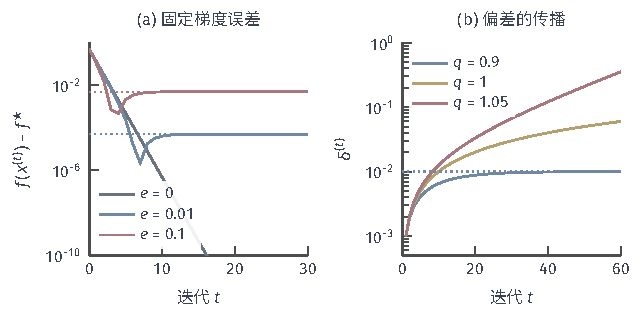
\includegraphics[width=108.5mm]{figures/03-optimization-evolution-and-signals/01-optimization/tikz/c3-error-propagation/figure.pdf}
  \caption{计算误差的影响。(a) $f(x)=x^2/2$上$\eta=1/2$、$x^{(0)}=1$的梯度下降，每步梯度带固定误差$e$；$e>0$时目标停在点线所示的$e^2/2$。(b) 递推$\delta^{(t+1)}=q\,\delta^{(t)}+10^{-3}$的解：$q=0.9$时趋于$0.01$（点线），$q=1$时线性增长，$q=1.05$时指数增长。}
  \label{fig:opt-smooth-error-propagation}
\end{figure}

\paragraph{传播系数从哪里来}
系数$q$由目标的曲率决定。设$f$二阶连续可微，则$T(\bm x)-T(\bm y)=(\bm I-\eta\bar{\bm H})(\bm x-\bm y)$，其中$\bar{\bm H}=\int_0^1\nabla^2f(\bm y+s(\bm x-\bm y))\,\mathrm ds$是线段上的平均Hessian。若沿途$\mu\bm I\preceq\nabla^2f\preceq L\bm I$，则$\bar{\bm H}$的特征值也在$[\mu,L]$中，
\[
  q\leq\max\{|1-\eta\mu|,\ |1-\eta L|\}.
\]
强凸（$\mu>0$）且$0<\eta<2/L$时$q<1$，更新映射是压缩映射；仅凸（$\mu=0$）且$0<\eta\leq2/L$时只有$q\leq1$，误差不衰减；一般的$L$光滑目标只能保证$q\leq1+\eta L$，负曲率方向上偏差会被放大。步长变化时要检查乘积$\prod_t q^{(t)}$，而不是每一项：逐项小于$1$不足以让旧误差消失，例如$q^{(t)}=1-1/(t+2)^2$时乘积趋于$1/2$。

带动量的方法要比较完整的状态。重球法的状态是$(\bm x^{(t)},\bm x^{(t-1)})$，在二次目标上状态按一个$2\times2$分块矩阵演化；这个矩阵的谱半径小于$1$保证误差最终衰减，但它不是对称矩阵，其范数可能大于$1$，偏差在衰减之前可以先短暂增长。两条轨迹即使当前参数$\bm x^{(t)}$相同，只要上一步的位移不同，下一步也会不同。本节只比较离散迭代之间的偏差；把迭代看成连续梯度流$\dot{\bm x}=-\nabla f(\bm x)$的离散化，并研究两者之间的误差，属于本卷第~\ref{part:dynamical-systems-control-decision-and-games}部分“过程与轨迹演化”的内容。

\section{最优解的敏感性}
\label{sec:opt-smooth-sensitivity}

上一节固定问题，研究算法返回的点离真正的最优解有多远。但目标中的数据往往来自测量或估计，本身就有误差。即使算法把手中的问题解得完全精确，所得的也只是“带误差数据的问题”的最优解。本节改变目标中的数据或参数，比较各个问题被精确求解后的最优解，判断问题本身对数据是否敏感。这是问题的性质，与用什么算法无关。

\subsection{扰动问题与解映射}
\label{sec:opt-smooth-solution-map}

\paragraph{一族问题}
设参数$\bm b$取值于某个集合，对每个$\bm b$给定$\mathbb R^d$上的可微目标$f_{\bm b}$。每个$\bm b$对应一个不同的无约束优化问题$\min_{\bm x}f_{\bm b}(\bm x)$，记其最优解集为$S(\bm b)=\argmin_{\bm x}f_{\bm b}(\bm x)$。映射$\bm b\mapsto S(\bm b)$称为\term{解映射}（solution map）。研究敏感性，就是比较$S(\bm b)$与$S(\bm c)$：两个不同问题的精确最优解。这与上一节的比较对象不同，那里比较的是同一个问题上的理想迭代与实际迭代，两者都还没有收敛到最优解。

\paragraph{三种误差的区分}
以二次目标族$f_{\bm b}(\bm x)=\tfrac12\bm x^\top\bm H\bm x-\bm b^\top\bm x$为例，$\bm H\succ\bm0$，唯一解为$\bm x_{\bm b}=\bm H^{-1}\bm b$。设真实数据是$\bm b$，手中只有带误差的$\bm b+\delta\bm b$，算法在后者上返回$\tilde{\bm x}$。三角不等式把总误差拆成两部分：
\[
  \lVert\tilde{\bm x}-\bm x_{\bm b}\rVert_2\leq\underbrace{\lVert\tilde{\bm x}-\bm x_{\bm b+\delta\bm b}\rVert_2}_{\text{算法求解误差}}+\underbrace{\lVert\bm x_{\bm b+\delta\bm b}-\bm x_{\bm b}\rVert_2}_{\text{数据误差引起的解变化}} .
\]
第一项可以通过多迭代几步缩小；第二项只取决于问题，算法再精确也去不掉。取$\bm H=\operatorname{diag}(1,0.1)$、$\bm b=(1,0.1)^\top$，解为$(1,1)^\top$；若$b_2$测成$0.2$，误差只有$0.1$，解却变为$(1,2)^\top$，移动了$1$。同样的数据误差作用在$\bm H=\bm I$上，解只从$(1,1)^\top$移到$(1,1.1)^\top$。图~\ref{fig:opt-smooth-sensitivity}画出了这两种情形：曲率小的方向上，等高线又长又平，线性项的一点改变就把碗底推出很远。

\begin{figure}[htbp]
  \centering
  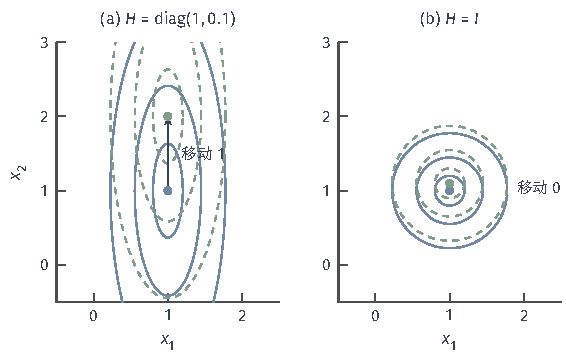
\includegraphics[width=95.8mm]{figures/03-optimization-evolution-and-signals/01-optimization/tikz/c3-sensitivity/figure.pdf}
  \caption{二次目标$f_{\bm b}(\bm x)=\tfrac12\bm x^\top\bm H\bm x-\bm b^\top\bm x$在数据改变前（蓝色实线）与改变后（绿色虚线）的等高线及最小点，两图中$b_2$都增加$0.1$。(a) $\bm H=\operatorname{diag}(1,0.1)$：$x_2$方向曲率只有$0.1$，最小点从$(1,1)$移到$(1,2)$，移动$1$。(b) $\bm H=\bm I$：最小点从$(1,1)$移到$(1,1.1)$，移动$0.1$。}
  \label{fig:opt-smooth-sensitivity}
\end{figure}

\paragraph{多解时先约定比较什么}
解不唯一时，“最优解怎样变化”需要先约定比较的对象。取$\bm H=\operatorname{diag}(1,0)$，它半正定而不正定。$\bm b=(1,0)^\top$时，$f_{\bm b}=\tfrac12x_1^2-x_1$，解集是整条直线$\{(1,s):s\in\mathbb R\}$；若约定选范数最小的解，得到$(1,0)^\top$。把数据改成$\bm b=(1,\epsilon)^\top$，$\epsilon\neq0$，目标多出一项$-\epsilon x_2$，沿$x_2$方向无下界，最优解根本不存在。无论$\epsilon$多小，解映射都从“一条直线”跳到“空集”。所以在多解问题中，不能不加约定就把最优解写成数据的单值连续函数：要么比较整个解集（例如用集合之间的距离），要么固定一个选解规则（例如最小范数），并分别检查这个规则下的解是否存在、是否连续。由数据选择函数时的选解问题在第~\ref{chap:opt-function-fitting}章展开。

\subsection{强凸目标的扰动界}
\label{sec:opt-smooth-strongly-convex-perturbation}

上面的例子提示，曲率的下界决定了解对线性扰动的敏感程度。下面把这一点写成一般结论。

\paragraph{线性扰动下的解变化}
第~\ref{chap:optimization}章的强凸一阶下界可以写成两个方向，再相加：对$\mu$强凸的可微函数$f$和任意$\bm x,\bm y$，
\[
  \begin{gathered}
  f(\bm y)\geq f(\bm x)+\langle\nabla f(\bm x),\bm y-\bm x\rangle+\frac\mu2\lVert\bm y-\bm x\rVert_2^2,\\
  f(\bm x)\geq f(\bm y)+\langle\nabla f(\bm y),\bm x-\bm y\rangle+\frac\mu2\lVert\bm x-\bm y\rVert_2^2 ,
  \end{gathered}
\]
相加得
\begin{equation}
\label{eq:opt-smooth-strong-monotone}
  \langle\nabla f(\bm x)-\nabla f(\bm y),\bm x-\bm y\rangle\geq\mu\lVert\bm x-\bm y\rVert_2^2 .
\end{equation}
这个性质称为梯度的\term{强单调性}（strong monotonicity）：梯度之差在位移方向上的投影，至少与位移的长度平方成正比。

\begin{theorem}[线性扰动下的解变化界]
\label{thm:opt-smooth-perturbation-bound}
设$f:\mathbb R^d\to\mathbb R$可微且$\mu$强凸（$\mu>0$），对$\bm b\in\mathbb R^d$令$f_{\bm b}(\bm x)=f(\bm x)-\langle\bm b,\bm x\rangle$。则每个$f_{\bm b}$有唯一最小点$\bm x_{\bm b}$，并且对任意$\bm b,\bm c$，
\[
  \lVert\bm x_{\bm b}-\bm x_{\bm c}\rVert_2\leq\frac1\mu\lVert\bm b-\bm c\rVert_2 .
\]
\end{theorem}

\begin{proof}
减去线性函数不改变强凸常数，所以$f_{\bm b}$仍是$\mu$强凸的；由第~\ref{chap:optimization}章，有限维上可微的强凸函数存在唯一最小点，且最小点处梯度为零，即$\nabla f(\bm x_{\bm b})=\bm b$，$\nabla f(\bm x_{\bm c})=\bm c$。代入式~\eqref{eq:opt-smooth-strong-monotone}，再用Cauchy--Schwarz不等式：
\[
  \mu\lVert\bm x_{\bm b}-\bm x_{\bm c}\rVert_2^2\leq\langle\bm b-\bm c,\bm x_{\bm b}-\bm x_{\bm c}\rangle\leq\lVert\bm b-\bm c\rVert_2\lVert\bm x_{\bm b}-\bm x_{\bm c}\rVert_2 .
\]
$\bm x_{\bm b}\neq\bm x_{\bm c}$时两边除以$\lVert\bm x_{\bm b}-\bm x_{\bm c}\rVert_2$即得结论，相等时结论显然。
\end{proof}

界中的$1/\mu$是精确的。对二次目标$\bm x_{\bm b}=\bm H^{-1}\bm b$，扰动沿最小特征值$\mu$的特征方向时，解的变化恰为$\lVert\delta\bm b\rVert_2/\mu$；图~\ref{fig:opt-smooth-sensitivity}(a)正是这种情形，$\mu=0.1$，扰动$0.1$造成移动$1$。解唯一并不意味着解稳定：$\mu$很小时，唯一的解可以对数据极为敏感。

\paragraph{绝对放大与条件数}
$1/\mu$度量的是绝对放大：数据改变一个单位，解最多改变多少个单位。它依赖于数据的尺度。另一种度量是相对的：对正定二次目标，由$\lVert\bm b\rVert_2\leq\lambda_{\max}\lVert\bm x_{\bm b}\rVert_2$与$\lVert\delta\bm x\rVert_2\leq\lVert\delta\bm b\rVert_2/\lambda_{\min}$，
\[
  \frac{\lVert\delta\bm x\rVert_2}{\lVert\bm x_{\bm b}\rVert_2}\leq\kappa(\bm H)\,\frac{\lVert\delta\bm b\rVert_2}{\lVert\bm b\rVert_2},\qquad\kappa(\bm H)=\frac{\lambda_{\max}(\bm H)}{\lambda_{\min}(\bm H)} .
\]
\term{条件数}（condition number）$\kappa$度量相对误差的放大，与整体尺度无关。两种度量回答不同的问题：$\bm H=\epsilon\bm I$的条件数是$1$，相对误差不放大，绝对误差却放大$1/\epsilon$倍。线性方程的条件数及其误差分析，参见本章前面引用的卷一“谱和奇异值”章。

\paragraph{问题的病态与算法的稳定}
本节的敏感性与上一节的误差传播是两件事。上一节的传播系数$q$描述算法在同一个问题上怎样处理执行误差，它取决于步长等算法选择；本节的$1/\mu$与$\kappa$描述问题本身，与算法无关。在病态问题上，再精确的算法也只能给出带误差数据所对应的最优解，提高求解精度不能消除问题自身的病态；要减小这部分误差，只能改善数据，或者改变问题本身，例如加入正则化项，这在第~\ref{chap:opt-function-fitting}章讨论。还要注意，本节只处理无约束目标中线性项的扰动。约束边界随数据移动、起作用的约束集合发生切换时，解可能不连续地跳动，需要第~\ref{chap:constrained-optimization}章的乘子与对偶工具来分析。

\section{本章小结}
\label{sec:opt-smooth-summary}

章首的问题是：在$f(\bm x)=\tfrac12(x_1^2+16x_2^2)$上，只凭一个点的目标值和梯度，怎样决定方向与步长，怎样保证下降，何时值得读取曲率，返回的点有多准、花了多少代价。本章的回答围绕一条线索：在当前点用局部模型代替目标，并时刻知道模型与真实目标差多少。

梯度Lipschitz条件给出了最基本的模型：一个曲率为$L$、盖住目标的二次上界。它的最小点就是步长$1/L$的梯度步，下降引理把“沿负梯度走足够小的一步”变成可计算的保证。由此得到三层结论：$L$光滑且下有界时，梯度下降使历史最佳梯度以$O(T^{-1/2})$减小；再加凸性与最小点存在，最后一点的目标差以$O(1/T)$减小；满足PL条件时目标差线性收敛。回溯线搜索在不知道$L$时用实际函数值完成同样的工作。统一常数$L$的代价是对平坦方向过于保守：共同例中曲率相差$16$倍，固定步长只能在“之”字与缓慢之间折中。

改进有两条路。一条是改变坐标或记住历史：固定预条件等价于换坐标后的梯度下降，好坏由变换后的曲率决定；重球法在二次目标上把依赖$\kappa$的收缩变为依赖$\sqrt\kappa$，Nesterov方法在一般凸光滑目标上把$O(1/T)$变为$O(1/T^2)$，代价是目标值不再单调。另一条是把曲率放进模型：牛顿法在非退化最小点附近二次收敛，但需要Hessian正定、需要线搜索控制远处的步长，每轮代价高；修正牛顿、信赖域与立方正则化分别用改曲率、限半径、加立方项的方式保证模型可用；Newton--CG只用Hessian向量积求解模型，拟牛顿用梯度差拼出曲率，它们降低每轮代价，也相应改变了能保证的局部速度。

非凸目标上，梯度小只说明接近某个驻点。严格鞍点处有负曲率方向，可以用二阶信息直接下降，也可以用扰动梯度下降在有限步内高概率地离开；但近似二阶驻点仍不等于局部最小点，更不等于全局最小点。比较算法时，误差对象、返回点、条件与成本口径必须一致：局部收敛阶不代表全程成本，每轮便宜也不代表总成本低。计算误差给可达精度设下了下限，而数据误差引起的解变化由问题自身的曲率下界决定，再精确的求解也无法消除。

表~\ref{tab:opt-smooth-summary}汇总了本章主要方法每轮使用的信息、所需条件与代价。

\begin{table*}[htbp]
  \centering
  \small
  \begin{tabularx}{\linewidth}{@{}>{\raggedright\arraybackslash}p{0.15\linewidth}>{\raggedright\arraybackslash}p{0.2\linewidth}>{\raggedright\arraybackslash}X>{\raggedright\arraybackslash}p{0.2\linewidth}@{}}
    \toprule
    方法 & 每轮使用的信息 & 主要保证及其条件 & 每轮主要代价（稠密$d$维） \\
    \midrule
    梯度下降 & 梯度；回溯时加函数值 & $L$光滑：残差$O(T^{-1/2})$；凸：目标差$O(1/T)$；PL：线性 & 一次梯度，$O(d)$存储 \\
    固定预条件 & 梯度与固定的$\bm P$ & 等价于新坐标中的梯度下降，速度由变换后曲率决定 & 应用$\bm P$的代价 \\
    重球法 & 梯度与上一步位移 & 正定二次、谱界已知：因子$\tfrac{\sqrt\kappa-1}{\sqrt\kappa+1}$ & 一次梯度，多存一个向量 \\
    Nesterov方法 & 前瞻点的梯度 & 凸、$L$光滑、最小点存在：目标差$O(1/T^2)$ & 一次梯度，多存一个向量 \\
    牛顿法 & 梯度与Hessian & 非退化最小点邻域：二次收敛；远处需线搜索 & $O(d^3)$分解，$O(d^2)$存储 \\
    信赖域 & 梯度与模型矩阵 & Cauchy下降、模型有界、下有界：梯度趋零 & 子问题求解，拒绝时重解 \\
    Newton--CG & 梯度与Hessian向量积 & 局部阶由强迫序列决定 & $k$次Hessian向量积，$O(d)$存储 \\
    BFGS／L-BFGS & 梯度与历史位移、梯度差 & 曲率条件下保持正定；完整BFGS局部超线性 & $O(d^2)$／$O(rd)$ \\
    立方正则化 & 梯度与Hessian & Hessian Lipschitz、下有界：$O(\varepsilon^{-3/2})$轮 & 子问题可达$O(d^3)$ \\
    扰动梯度下降 & 梯度与随机扰动 & 高概率返回近似二阶驻点 & 一次梯度，偶尔一次函数值 \\
    \bottomrule
  \end{tabularx}
  \caption{本章主要方法的比较。各行保证的误差对象和条件不同，只能在列出的条件下解读，不构成方法之间的无条件排序。}
  \label{tab:opt-smooth-summary}
\end{table*}

本章始终假设目标可微、没有约束、梯度可以精确地对整个目标求出。后续各章依次放松这些假设：第~\ref{chap:opt-nonsmooth}章处理尖点和由几项组成的复合目标，那里下降引理与邻近映射一起构成新的局部模型；第~\ref{chap:constrained-optimization}章处理可行范围，并在内点法中再次用到牛顿法；第~\ref{chap:opt-stochastic-block}章处理只能抽样得到的梯度和分块更新。多解问题中由数据和算法共同决定选出哪个解，集中在第~\ref{chap:opt-function-fitting}章讨论。

